\section{Applications}

\subsection{Denoising \cite{coupe_2008}}

\begin{description}
 \item[btkNLMDenoising] This program applies a non-local mean filter to a 3D
image  for denoising purpose. Usage: \texttt{-i ana.nii.gz -o ana\_nlm.nii.gz }
. The best results are usually obtained by using a mask
(or a padding value). This is an implementation of the method proposed by Coup\'e \textit{et al.} in \cite{coupe_2008}.
\end{description}

\begin{description}
 \item[btkNLMDenoising4DImage] This program applies a non-local mean filter to 
 each 3D image of a 4D image, for denoising purpose. Usage: \texttt{-i dwi.nii.gz -o dwi\_nlm.nii.gz }. The best results are usually
obtained by using a mask (or a padding value).
\end{description}


\subsection{Anatomical reconstruction}
\label{subsec:ana_rec}

\begin{description}
 \item[btkImageReconstruction] This program allows to obtain a
high-resolution image from a set of low-resolution images, typically
axial, coronal, and sagittal acquisitions~(similar to \cite{rousseau_registration_2006}). \\\\
Minimal usage: \texttt{btkImageReconstruction -i ana01.nii.gz $\cdots$ -i anaN.nii.gz \\\ -o
ana\_reconstructed.nii.gz --box}. 

Recommended usage: \texttt{btkImageReconstruction -i ana01.nii.gz $\cdots$ -i anaN.nii.gz\\
-m mask01.nii.gz $\cdots$ -m maskN.nii.gz -o ana\_reconstructed.nii.gz --mask}. 

The use of a mask provide better results since it allows an accurate estimation of the initial
transform, and constrains the registration to the region of interest.

The full list of optional parameters of the method can be obtained by
\texttt{btkImageReconstruction --help}

\end{description}

\begin{description}
 \item[btkSuperResolution] To be documented. 

\end{description}

\subsection{Anatomical segmentation}
\label{subsec:ana_seg}

\begin{description}
 \item[btkTissueSegmentation] This program allows to obtain :
        \begin{itemize}
         \item A segmentation of the brain which separate pericerebral LCR and ventricules,
         \item A segmentation of the cortex inside of a region of interest defined from the border between brain and pericerebral LCR,
        \end{itemize}
        as described in~\cite{caldairou_segmentation_2011}.
        
        Usage: \texttt{btkTissueSegmentation -i ana.nii.gz -s intracranian\_volume.nii.gz \\
        -l brainstem\_segmentation.nii.gz -l cerebellum\_segmentation.nii.gz \\
        -o brain\_segmentation.nii.gz -o cortex\_segmentation.nii.gz}
\end{description}

\begin{description}
 \item[btkLabelPropagation] This program applies a patch-based label propagation algorithm for segmentation~\cite{rousseau_supervised_2011}. As a supervised method, it takes as input a textbook containing several anatomical images and the corresponding segmentation maps.
\end{description}


\subsection{Reconstruction of DW sequences \cite{oubel_reconstruction_2010}}
\label{subsec:diff_rec}
The reconstruction of diffusion-weighted (DW) sequences aims at
obtaining a sequence corrected for fetal moving and eddy-current distortions.
This can be performed in BTK by using the two following applications. 
\begin{description}
\item[btkGroupwiseS2SDistortionCorrection] It performs a groupwise
slice-by-slice registration of the image components of the sequence.

Minimal usage: \texttt{btkGroupwiseS2SDistortionCorrection -i dwi\_normalized.nii.gz \\
-o dwi\_reconstructed.nii.gz -t transform\_folder}.

\begin{itemize}
 \item[-i] dwi sequence noramlized (Utilities/btkSequenceNormalization).
 \item[-o] dwi sequence reconstructed.
 \item[-t] folder to save the transformation files
\end{itemize}

The slice-by-slice transform for a given DW image is saved as a set of $N$
transforms in ITK format, with $N$ the number of slices in the image.

NOTE: For slice registration, 20\% of the samples are used for computing the
image metric. As the region of interest of the slice can be small, this number
of samples might be insufficient to compute the metric accurately. However,
this percent of samples has been sufficient for the tested sequences. 

\item[btkRBFInterpolationS2S] It performs an interpolation of scattered data
generated from the application of slice-by-slice transforms. To this end,
radial basis functions are used. By default, the output has isotropic
voxels of size equal to the in-plane resolution of the input.

Minimal usage: \texttt{btkRBFInterpolationS2S -i dwi\_normalized.nii.gz -m mask.nii.gz \\
-o dwi\_interpolated.nii.gz -t transformation\_folder}.

\begin{itemize}
 \item[-i] dwi sequence normalized
 \item[-m] mask for the B0 image
 \item[-o] dwi sequence interpolated 
 \item[-t] folder with the transformations generated by
\texttt{btkGroupwiseS2SDistortionCorrection}
\end{itemize}

\end{description}


\subsection{Tractography \cite{pontabry_probabilistic_2011}}
\label{subsec:tracto}

    \subsubsection*{Standard usage}
        Suppose you want to perform a tractography on a diffusion weighted MRI 
dataset. You should have a dwi image, the corresponding gradient vectors'
coordinates, a mask of the brain white matter and a label image of the seeds.
Assume this data is stored in files named respectively for instance
\texttt{dwi.nii.gz}, \texttt{dwi.bval}, \texttt{dwi.bvec}, \texttt{mask.nii.gz} and
\texttt{seeds.nii.gz}. The tractography is accomplished by the command below.
            \begin{quote}
                \texttt{btkTractography -d dwi.nii.gz -m mask.nii.gz -r seeds.nii.gz}
            \end{quote}
        When the program terminates its task, the probability connection map and
        the fibers estimation are saved in files respectively named
\texttt{map.nii.gz} and \texttt{fibers.vtk}. The connection map is a volume
image of probability intensities (\texttt{i.e.} intensities between 0 and 1)
with the same origin, orientation and spacing as the diffusion weighted image.
The fibers are polygonal data of VTK library in world coordinates.
%The standard
%pipeline of the program is shown in
%Fig.~\ref{btkTractography-fig:standard-pipeline}.
%            \begin{figure}
%                \centering
%                \includegraphics[width=0.6\textwidth]{btkTractographyPipeline}
%                \caption{Standard pipeline of the btkTractography program.}
%                \label{btkTractography-fig:standard-pipeline}
%            \end{figure}

        The file named \texttt{seeds.nii.gz} is a label map which is used to 
        generate seeds for the algorithm. The spacing in millimeters between
seeds can be adjust with the option \texttt{-\hspace{0.1mm}-seed\_spacing}.

        Before doing anything, be sure that the diffusion sequence has been normalized by using the utility \texttt{btkDiffusionSequenceNormalization}.
        
        This program contains three different algorithms: a tensor streamline, an fODF streamline and a fODF particle filtering algorithm. The choice of the model to use is achieved by using the option \texttt{--tensor}, which set the diffusion model to tensor model. The choice of the algorithm is achieved by using the option \texttt{--streamline}, which set the algorithm to use to the streamline one.

    \subsubsection*{Advanced usage}
        In addition to standard arguments of \texttt{btkTractography} program, 
        there are some other parameters that let you to alter algorithm's
behaviour. These options can be classified into three groups : model's options,
constraints on trajectory and tracking options. The first group options allow
you to tweak the model (for more details about fODF modeling, please refer
to~\cite{descoteaux_regularized_2007}). The second group options let you to
control the fiber trajectory. These options provide prior informations to
the algorithm. The last group options are dedicated to the tracking algorithm
control.

        Since the default parameters values may work in the most of cases, they 
        are optional. A list is of optional features is avaible by using the
command
            \begin{quote}
                \texttt{btkTractography -\hspace{0.1mm}-help} \hspace{0.5mm} or 
                \hspace{0.5mm} \texttt{btkTractography -h}
            \end{quote}
        and program's arguments are much more described below.


    \subsubsection*{Model's order (fODF only)}
        The model's order (i.e. the spherical harmonics' order) can be specified
        by the option
            \begin{quote}
                \texttt{-\hspace{0.1mm}-model\_order <order>} \enspace ,
            \end{quote}
        for \texttt{order}$\;\in\{2,4,6,8\}$. The default value is 4. For more 
        details, please refer to~\cite{descoteaux_regularized_2007}.

    \subsubsection*{Model's regularization (fODF only)}
        A Laplace-Beltrami regularization coefficient is used to assume a better
        estimation of the model. This coefficient can by manually modified by
the option
            \begin{quote}
                \texttt{-\hspace{0.1mm}-model\_regularization <coefficient>} \enspace ,
            \end{quote}
        for \texttt{coefficient}$\;\in\mathbb{R}$. The default value is set as 
        0.006. For more details, please refer
to~\cite{descoteaux_regularized_2007}.

    \subsubsection*{Displacement step size}
        The displacement step size of a moving particle can ben adjusted as you 
        want by using the option
            \begin{quote}
                \texttt{-\hspace{0.1mm}-step\_size <length>} \enspace ,
            \end{quote}
        where \texttt{length}$\;\in\mathbb{R}_+^*$. Note that this option is 
        expressed in~\texttt{mm}. The default value is fixed at 0.5~\texttt{mm}.
        By setting a big step size, the particles will move quickly. So the
biger is the step, the faster the algorithm will finish, but as shown by
Fig.~\ref{tracto-fig:stepSize}, some informations may be missed and the
particle's trajectories may overshoot the ground truth, resulting in a bad
estimation.

        \begin{figure}
            \centering
            \includegraphics[height=0.1\textheight]{stepSize}
            \caption{Effect of the step size option on a particle's trajectory. 
            With a large step size (right), the particle may overshoot the
trajectory of the ground truth.}
            \label{tracto-fig:stepSize}
        \end{figure}


    \subsubsection*{Angular threshold}
        An angular threshold prevent a particle to return back. This option has 
        to be expressed in radian and can bet set by
            \begin{quote}
                \texttt{-\hspace{0.1mm}-angular\_threshold <angle>} \enspace ,
            \end{quote}
        where \texttt{angle}$\;\in]0,2\pi[$. The default value is set as a 
        $\tfrac{\pi}{3}$ angle. As illustrated in two dimensions in
Fig.~\ref{tracto-fig:angleThreshold}, an angle threshold is used to define an
allowed area for successive sampled directions. This can be seen as a global
curvature parameters on trajectories. A small angle defines trajectories with a
small curvature. This is a prior information on ground truth trajectory.

        \begin{figure}
            \centering
            \includegraphics[height=0.1\textheight]{angleThreshold}
            \caption{An angle threshold allows the algorithm to sample
successive direction only in the cone defined by this angle. This
illustration show the principle in two dimensions.}
            \label{tracto-fig:angleThreshold}
        \end{figure}
        
    \subsubsection*{Trajectory interpolation method (streamline only)}
    
        When using streamline algorithm, by default the Runge-Kutta method at order~4 is used. The Euler's method can be used instead by setting the option \texttt{--no\_RK4}.


    \subsubsection*{Rigidity (particle filter only)}
        The rigidity option controls how much you want the particles to have 
        straight trajectory. You can adjust it by
            \begin{quote}
                \texttt{-\hspace{0.1mm}-curve\_constraint <rigidity>} \enspace ,
            \end{quote}
        where \texttt{rigidity}$\;\in\mathbb{R}_+^*$. The default value is
fixed at 30. This value correspond to a concentration parameter of a von
Mises-Fisher density probability used in the prior density of the system. As
Fig.~\ref{tracto-fig:concentration} illustrates locally in two dimensions, a
high value leads to a straight trajectory.

        \begin{figure}
            \centering
            \includegraphics[height=0.1\textheight]{concentration}
            \caption{Local effect of rigidity parameter on a particle's
trajectory. This parameter helps to ``attract'' the current
displacement vector in the direction of the previous displacement vector of a
particle. It correspond to a concentration paramter of a von Mise-Fisher density
probability used in the prior density of the system. For instance, a rigidity of
0 leads to an equiprobable distribution, whereas a rigidty tending to infinity
leads to a distribution focused on a point.}
            \label{tracto-fig:concentration}
        \end{figure}


    \subsubsection*{Number of particles (particle filter only)}
        The number of particles in the system is set by the option
            \begin{quote}
                \texttt{-\hspace{0.1mm}-number\_of\_particles <number>} \enspace ,
            \end{quote}
        where \texttt{number}$\;\in\mathbb{N}^*$. By default, the algorithm will
        use 1000 particles. A poor number of particles leads to a short
computation time and a poor estimation. A large number of particles leads to a
long computation time and a good estimation. In general, the default number of
particles is a good compromise between computation time and estimation.


    \subsubsection*{Resampling threshold (particle filter only)}
        This option modify the resampling threshold of the system. When the
number of effective particles in the system falls below this resampling
threshold, the particles are resampled according a multinomial resampling. It
can be adjust by
            \begin{quote}
                \texttt{-\hspace{0.1mm}-resampling\_threshold <percent>} \enspace ,
            \end{quote}
        where \texttt{percent}$\;\in[0,1]$ is the percent of minimal effective 
        particles in the system. A low threshold value will result in an
inefficient algorithm because the particles with low weight are not are not
often eliminated. Conversely, a high threshold value leads to a bad estimation
because the search space will not be explored enough.


\subsection{Atlas construction \cite{pontabry_2012_longitudinal}}
\label{subsec:atlas}

    There are two steps for atlas construction: filling the data script and building the atlas using the scripts. The following sections describe how you can do it.

    \subsubsection*{Filling the data script}
    
    The data script (\emph{btkAtlasData.py}) is used to give information to the executed script about the directories, the algorithms' options, which image modalities are used, etc. It has to be customized according to the data you have.
    
    The atlas construction scripts take as input series of images (such as T2, label images, etc.), corresponding to the patients of the dataset. The input files should be named as \emph{patientIdentifier\_modalityIden\-tifier.nii.gz} and placed in the specified directory for the modality \emph{modalityIdentifier}. There are basically two use cases: 1) you do not have any label image or 2) you have a label image.

    If you are working without labels, and for instance you only have T2 image, you have to add the following piece of code in the modalities part of the script.
    \begin{verbatim}
        # T2 modality
        # Identifier of the modality is T2 (input will be patientIdentifier_T2.nii.gz)
        ModalityImage = 'T2'
        # Initialization
        modalities[ModalityImage] = {}
        # T2 images will be used during registration
        modalities[ModalityImage][UseInRegistration] = True
        # T2 images will be used during regression
        modalities[ModalityImage][UseInRegression]   = True
        # The weight of T2 images is 1
        modalities[ModalityImage][ModalityWeight]    = 1
        # The path of T2 images is /path/to/data/T2
        modalities[ModalityImage][ModalityDataPath]  = dataPath + '/T2'
        # T2 is not a label
        modalities[ModalityImage][IsTissueMap]       = False
        # T2 is not a label, this field does not matter
        modalities[ModalityImage][TissueLabel]       = 0
    \end{verbatim}

    If you are working with labels, and for instance you have T2 images and labels images named \emph{patientIdentifier\_Tissues.nii.gz} in the data directory \emph{/path/to/data/Tissues}. Assume the label images contains 5 labels and you want to use only 2 labels (GM and WM). So you have to add the following piece of code in the modalities part of the script.
    \begin{verbatim}
        # T2 modality
        # Identifier of the modality is T2 (input will be patientIdentifier_T2.nii.gz)
        ModalityImage = 'T2'
        # Initialization
        modalities[ModalityImage] = {}
        # T2 images will be used during registration
        modalities[ModalityImage][UseInRegistration] = True
        # T2 images will be used during regression
        modalities[ModalityImage][UseInRegression]   = True
        # The weight of T2 images is 1
        modalities[ModalityImage][ModalityWeight]    = 1
        # The path of T2 images is /path/to/data/T2
        modalities[ModalityImage][ModalityDataPath]  = dataPath + '/T2'
        # T2 is not a label
        modalities[ModalityImage][IsTissueMap]       = False
        # T2 is not a label, this field does not matter
        modalities[ModalityImage][TissueLabel]       = 0
        
        # GM modality
        # Identifier of the modality is GM (input will be patientIdentifier_GM.nii.gz)
        ModalityImage = 'GM'
        # Initialization
        modalities[ModalityImage] = {}
        # GM images will be used during registration
        modalities[ModalityImage][UseInRegistration] = True
        # GM images will be used during regression
        modalities[ModalityImage][UseInRegression]   = True
        # The weight of GM images is 0.5
        modalities[ModalityImage][ModalityWeight]    = 0.5
        # The path of GM images is /path/to/data/GM
        modalities[ModalityImage][ModalityDataPath]  = dataPath + '/GM'
        # GM is a label
        modalities[ModalityImage][IsTissueMap]       = True
        # GM is the label 1
        modalities[ModalityImage][TissueLabel]       = 1
        
        # WM modality
        # Identifier of the modality is WM (input will be patientIdentifier_WM.nii.gz)
        ModalityImage = 'WM'
        # Initialization
        modalities[ModalityImage] = {}
        # WM images will be used during registration
        modalities[ModalityImage][UseInRegistration] = True
        # WM images will be used during regression
        modalities[ModalityImage][UseInRegression]   = True
        # The weight of WM images is 0.5
        modalities[ModalityImage][ModalityWeight]    = 0.5
        # The path of WM images is /path/to/data/WM
        modalities[ModalityImage][ModalityDataPath]  = dataPath + '/WM'
        # WM is a label
        modalities[ModalityImage][IsTissueMap]       = True
        # WM is the label 3
        modalities[ModalityImage][TissueLabel]       = 3
    \end{verbatim}

    
    \subsubsection*{Building atlas}

    Once the data script \emph{Scripts/btkAtlasData.py} has been copied in your working directory and filled according to the dataset and the algorithms' options (see previous section for some help), the atlas has to be built using dedicated scripts. First, the directory where the data script is have to be added in the python path environnement variable. For instance, in a terminal, the following command add the current directory in the python path environnement variable:
        \begin{quote}
            \texttt{export PYTHONPATH = \$PYTHONPATH:`pwd`} \enspace .
        \end{quote}
    Finaly, the atlas construction can be achieved by calling directly the following python scripts.

    \begin{description}
        \item[btkPrepareAtlasData] This optional script will split the tissue label map (if any and named \emph{patient-name\_Tissues.nii.gz}) into separate tissue probability maps. Tissue name and label are controlled by setting up the script \emph{Scripts/btkAtlasData.py}.

        Usage: \texttt{btkPrepareAtlasData.py}

        \item[btkCreateTemplate.py] This script will use the informations contained in the data script to produce a template normalization as output.

        Usage: \texttt{btkCreateTemplate.py}

        \item[btkCreateLongitudinalAtlas.py] This script will use the informations contained in the data script and the output of the script \emph{btkCreateTemplate.py} to produce a longitudinal atlas over gestionnal ages (in weeks) as output. So, the script \emph{btkCreateTemplate.py} must be executed before using this script.

        Usage: \texttt{btkCreateLongitudinalAtlas.py}
    \end{description}

\subsection{Mask Extraction}
\label{subsec:Mask}

Suppose you want to extract automicaly masks of your images. First of all you should have some Atlas of foetal brain for different ages (in week).
In Addition you should know age of every image you want to process.
The pipeline will registrate the corresponding age template with the current image, finaly you will have a new template succefully registrate on you image and you can use it as a mask.
The mask extraction can be achieved by calling directly the first following python script.
    \begin{description}
        \item[btkMaskExtraction.py] This script will contain all your images, you must edit it ! It contain examples. This script is the only one you should execute, it will automaticaly search and execute the second one.

        Usage: \texttt{btkMaskExtraction.py}

        \item[btkMaskExtractionProcess.py] This script will process the pipeline, you must edit the images\_directory and template\_directory. Note that your image directory should respect a hierarchy (written in the script).

        Usage: Should be run by btkMaskExtraction.py or for advance user you can call like this : \texttt{btkMaskExtractionProcess.py subject exam age image01 image02 ...}
    \end{description}

\subsection{Fiber tracts Clustering}
\label{subsec:clustering}

Fiber tracts clustering is used to map the well-known fiber bundles of white matter.
This can be performed using the following applications:

\begin{description}
        \item[btkProbabilisticSegmentationMapBasedClustering] As supervised method, this program takes as input a probabilistic segmentation MAP of brain tissue which is an 4D image in \href{http://nifti.nimh.nih.gov/nifti-1}{Nifti} format.\\

	Usage: \texttt{btkProbabilisticSegmentationMapBasedClustering -b fiber\_tractography.vtk -p 4D\_prob\_segmentation\_map.nii.gz -o fiber\_clustering.vtk}\\
 
	Fig.\ref{clustering1-fig} shows an example of clustering results obtained using the method above.

	\begin{figure}[h]
	\centering
        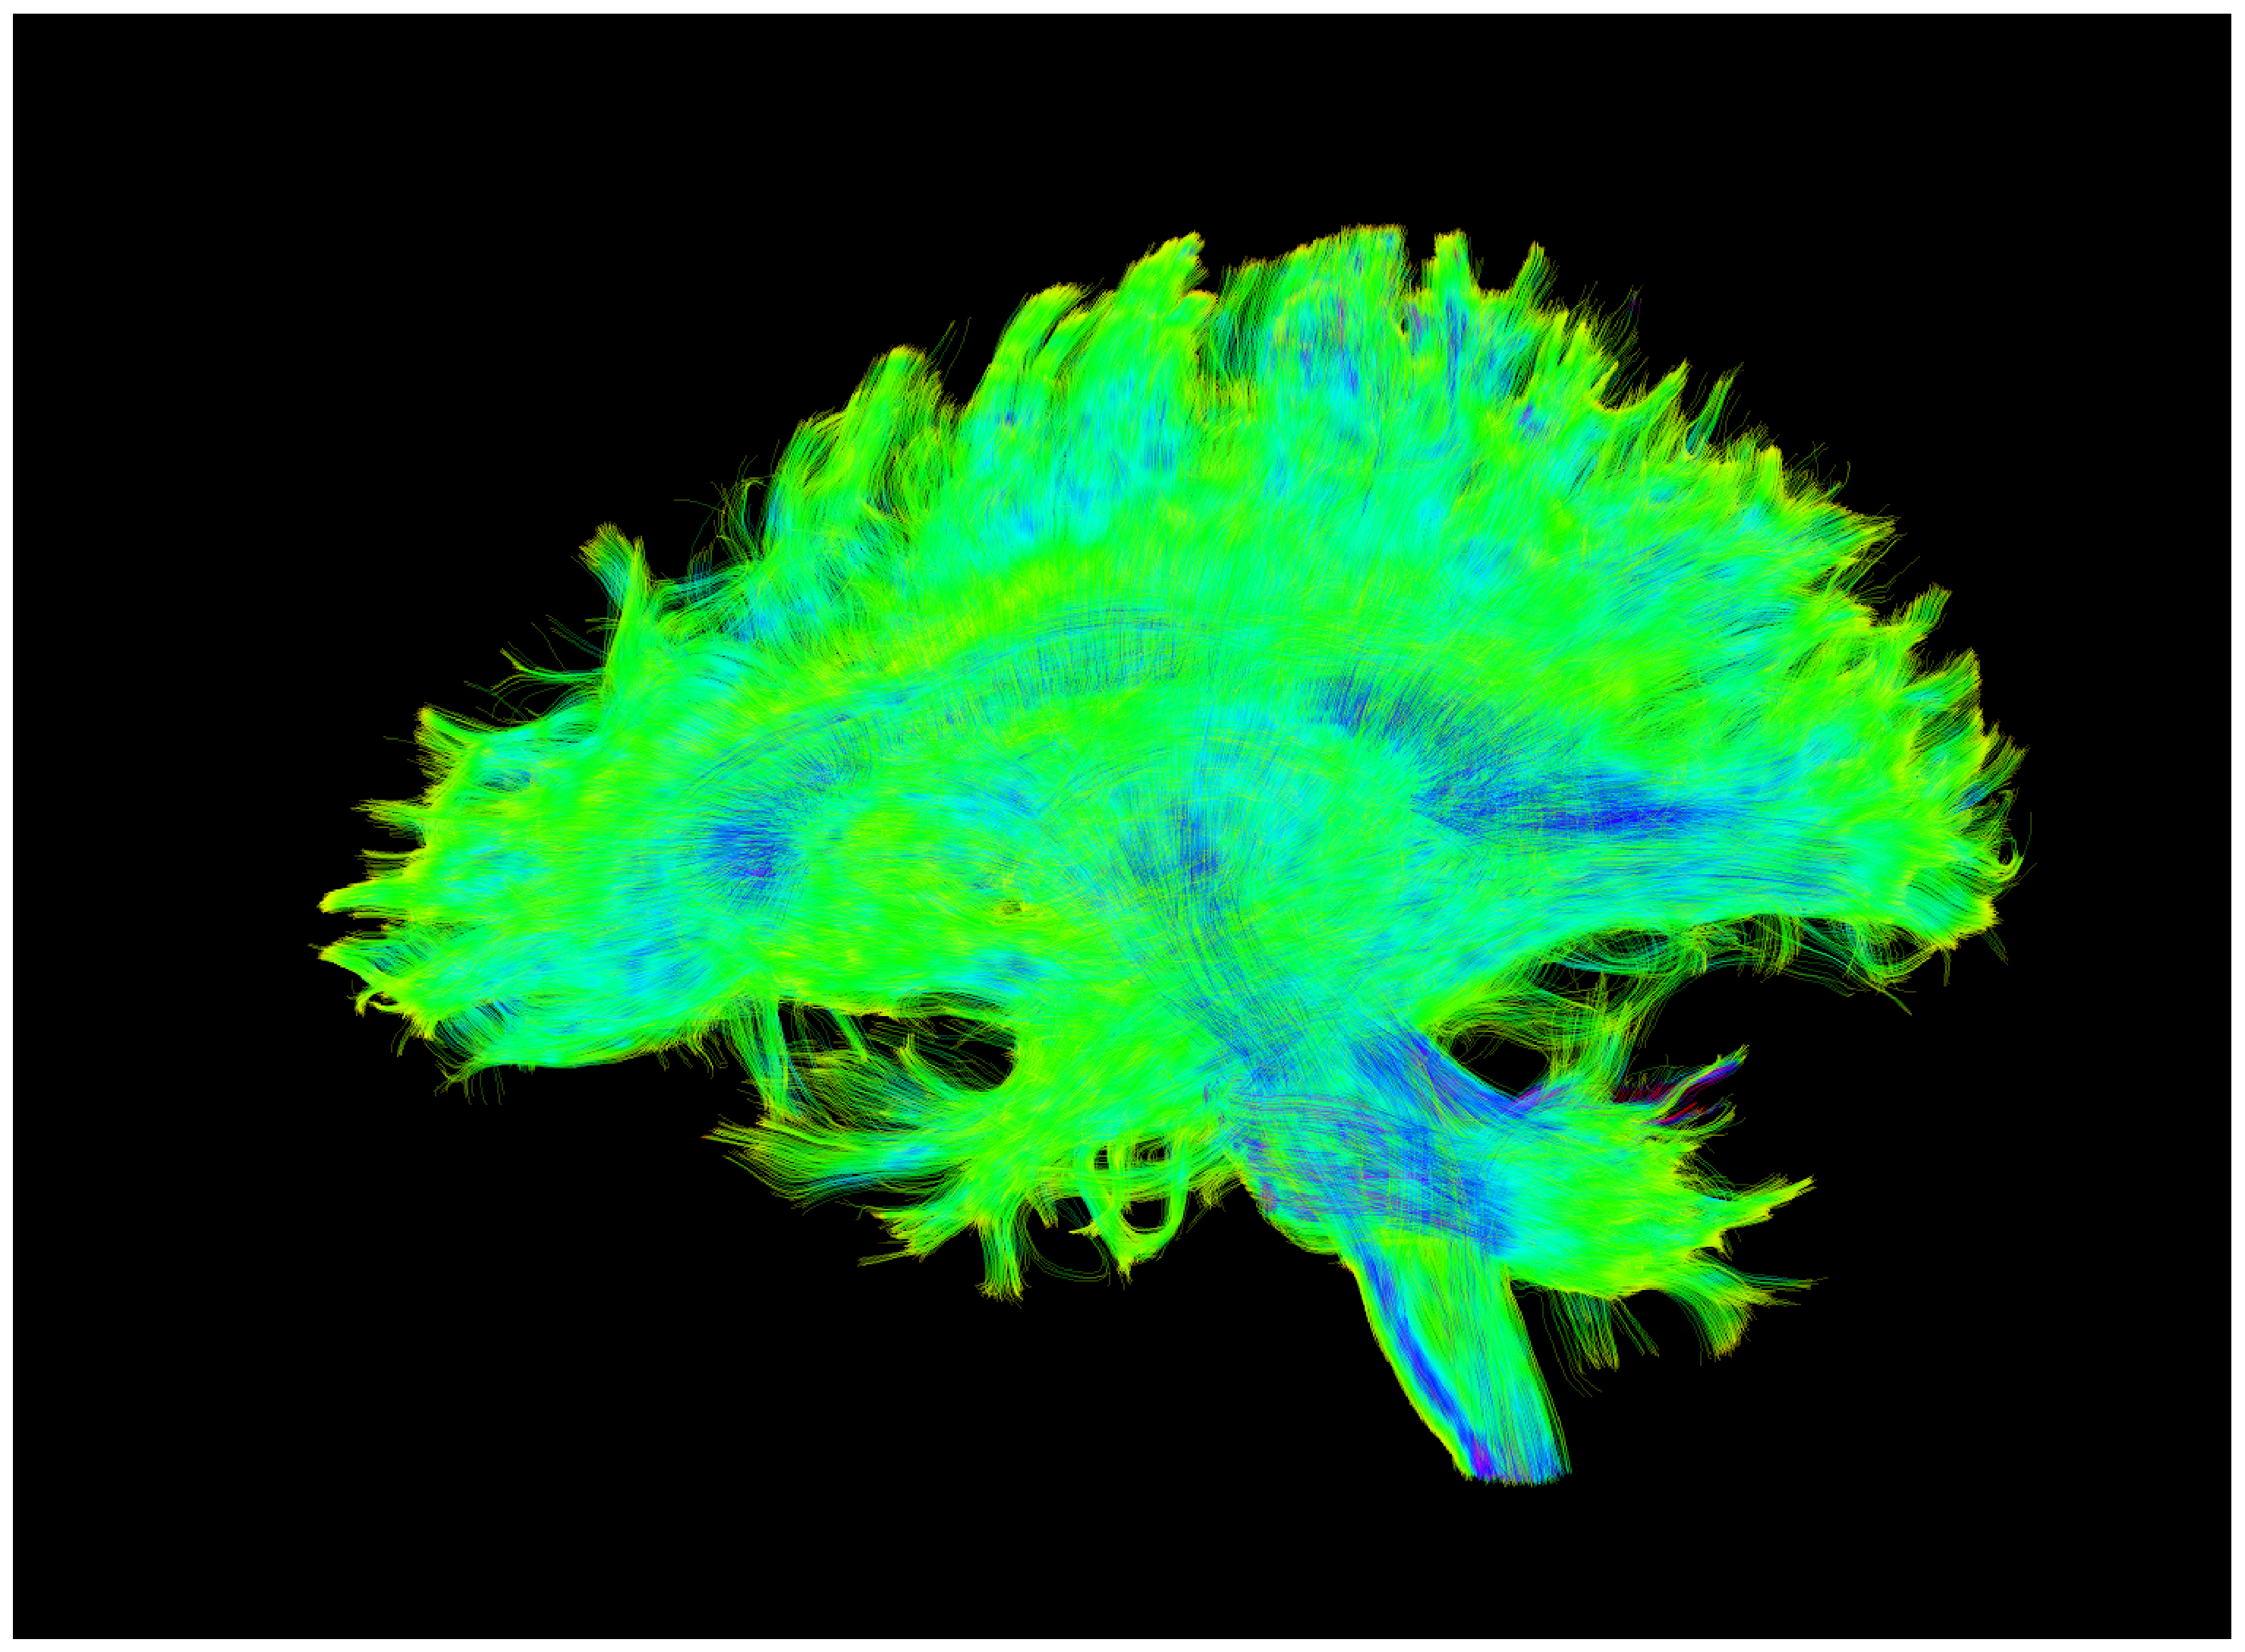
\includegraphics[width=4cm]{Tarctography1-Left-View}
        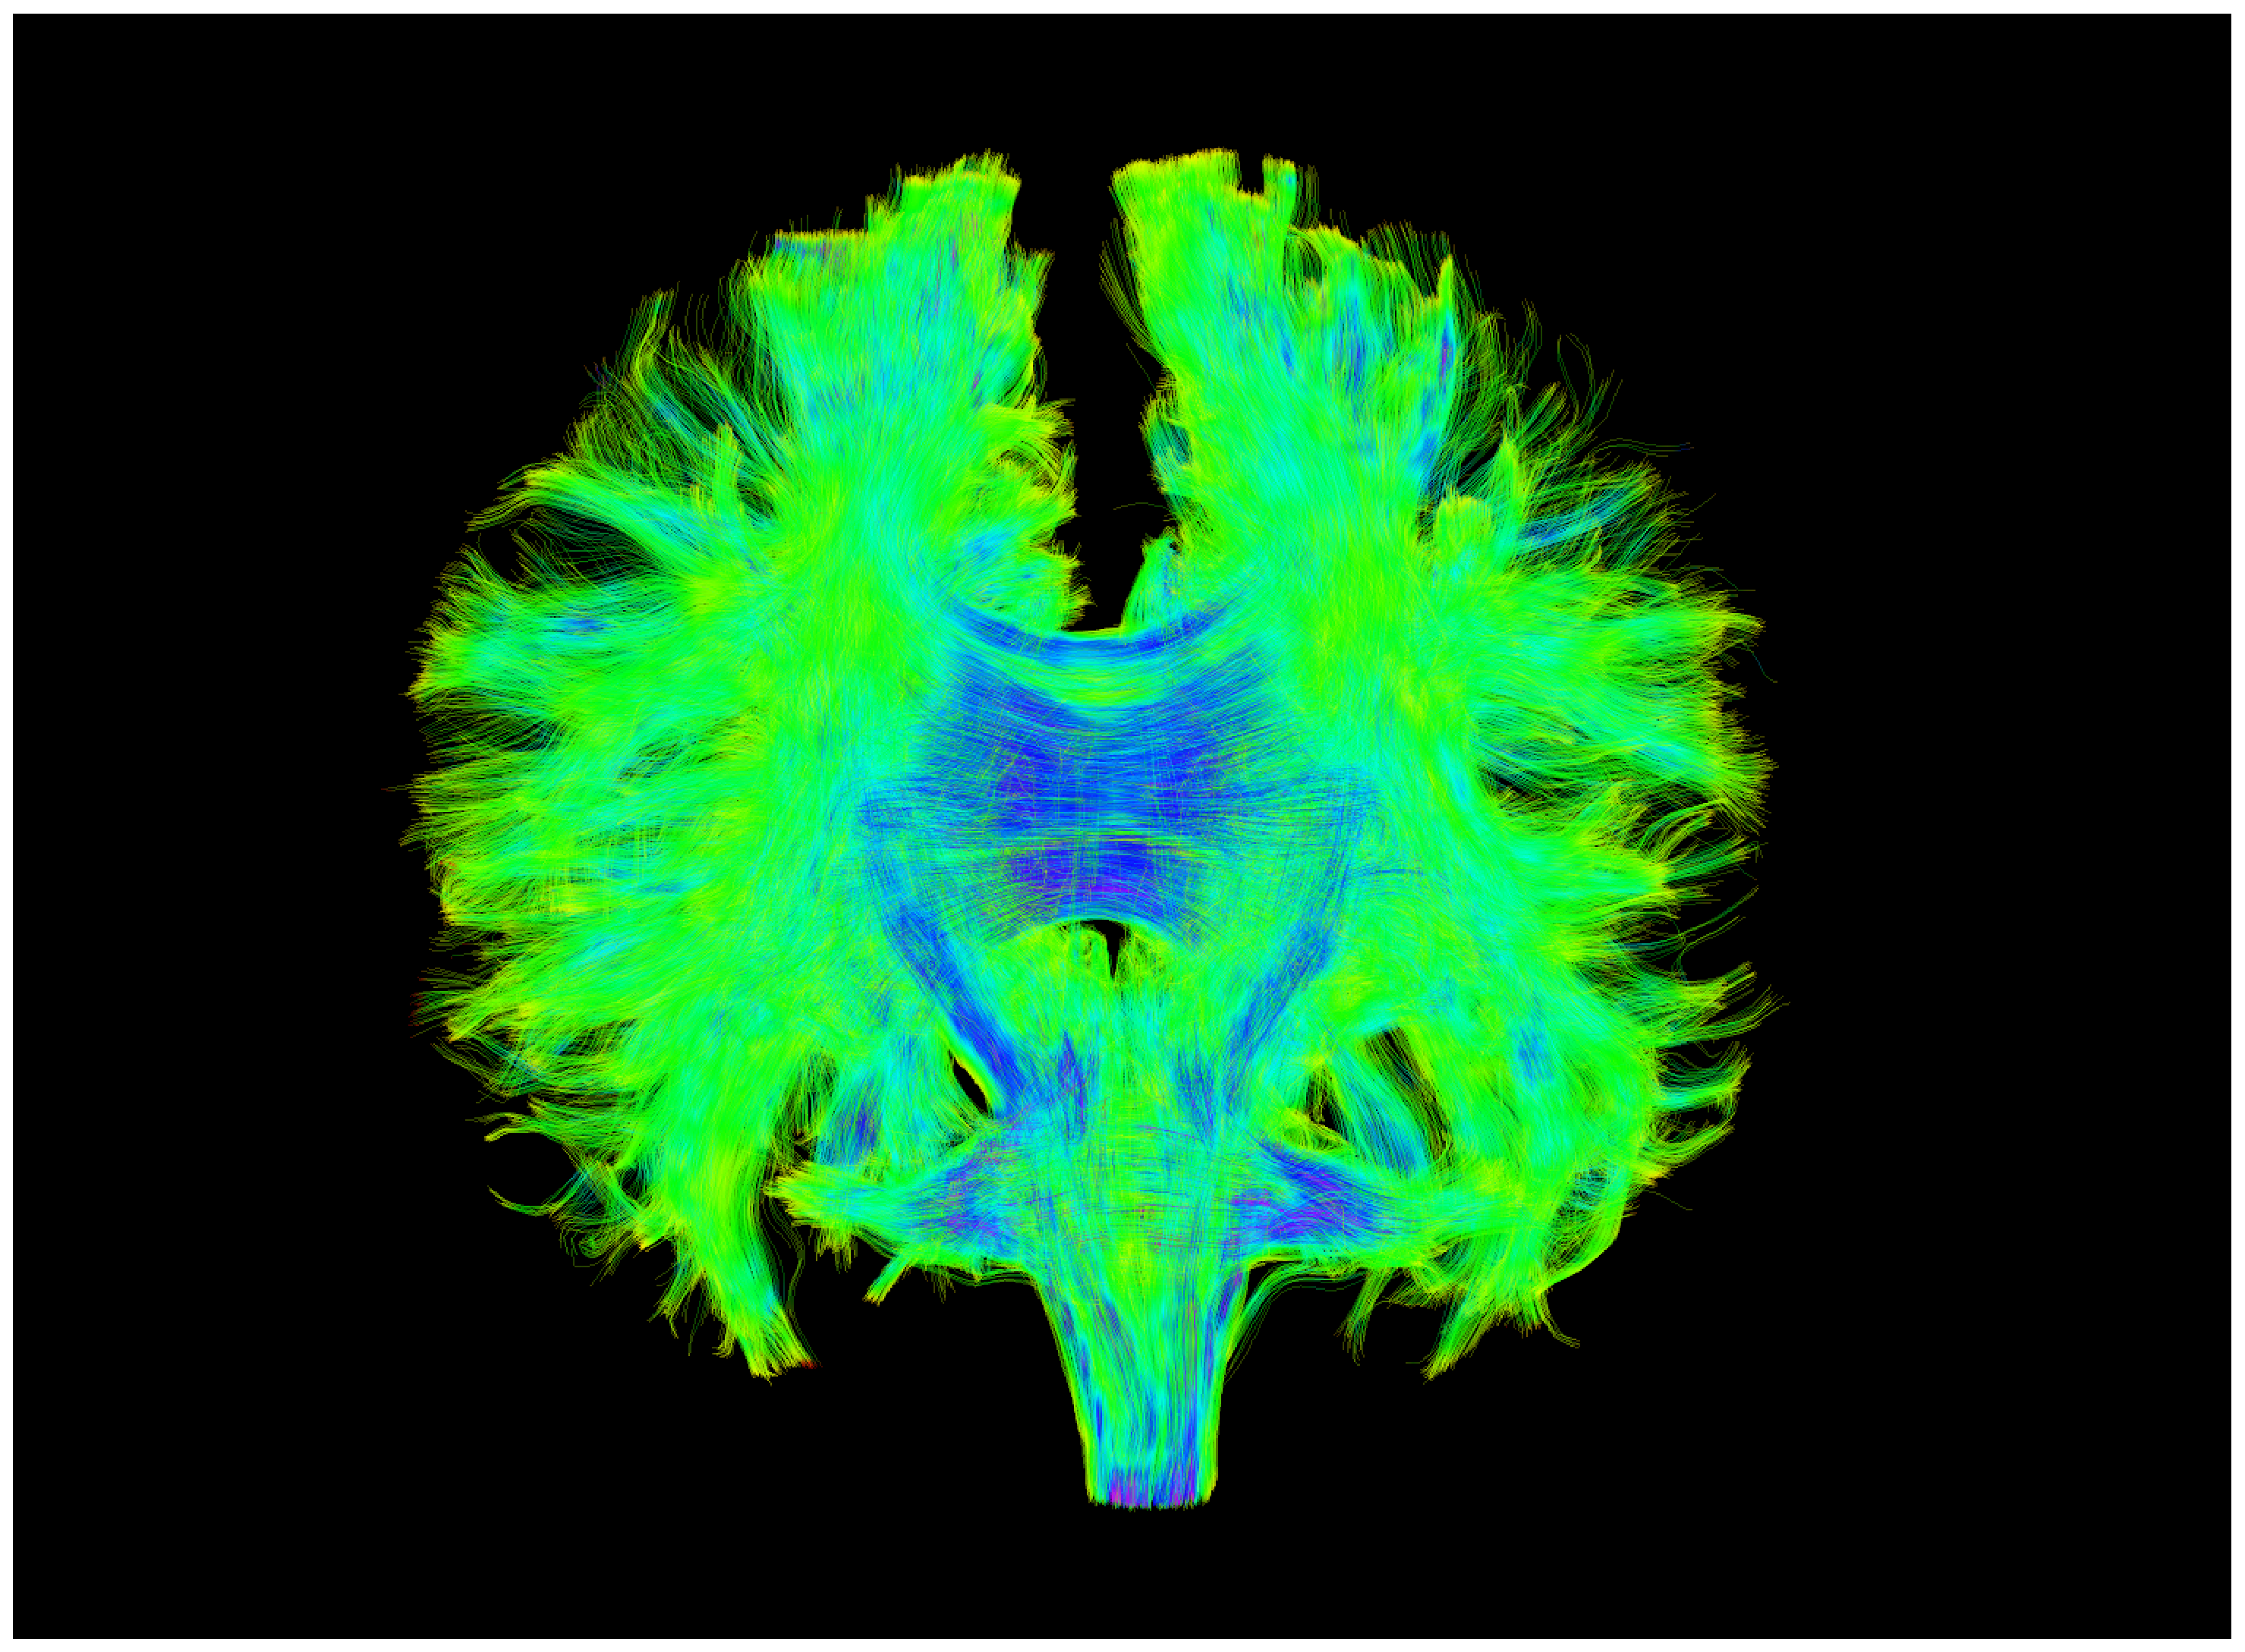
\includegraphics[width=4cm]{Tarctography1-Anterior-View}
        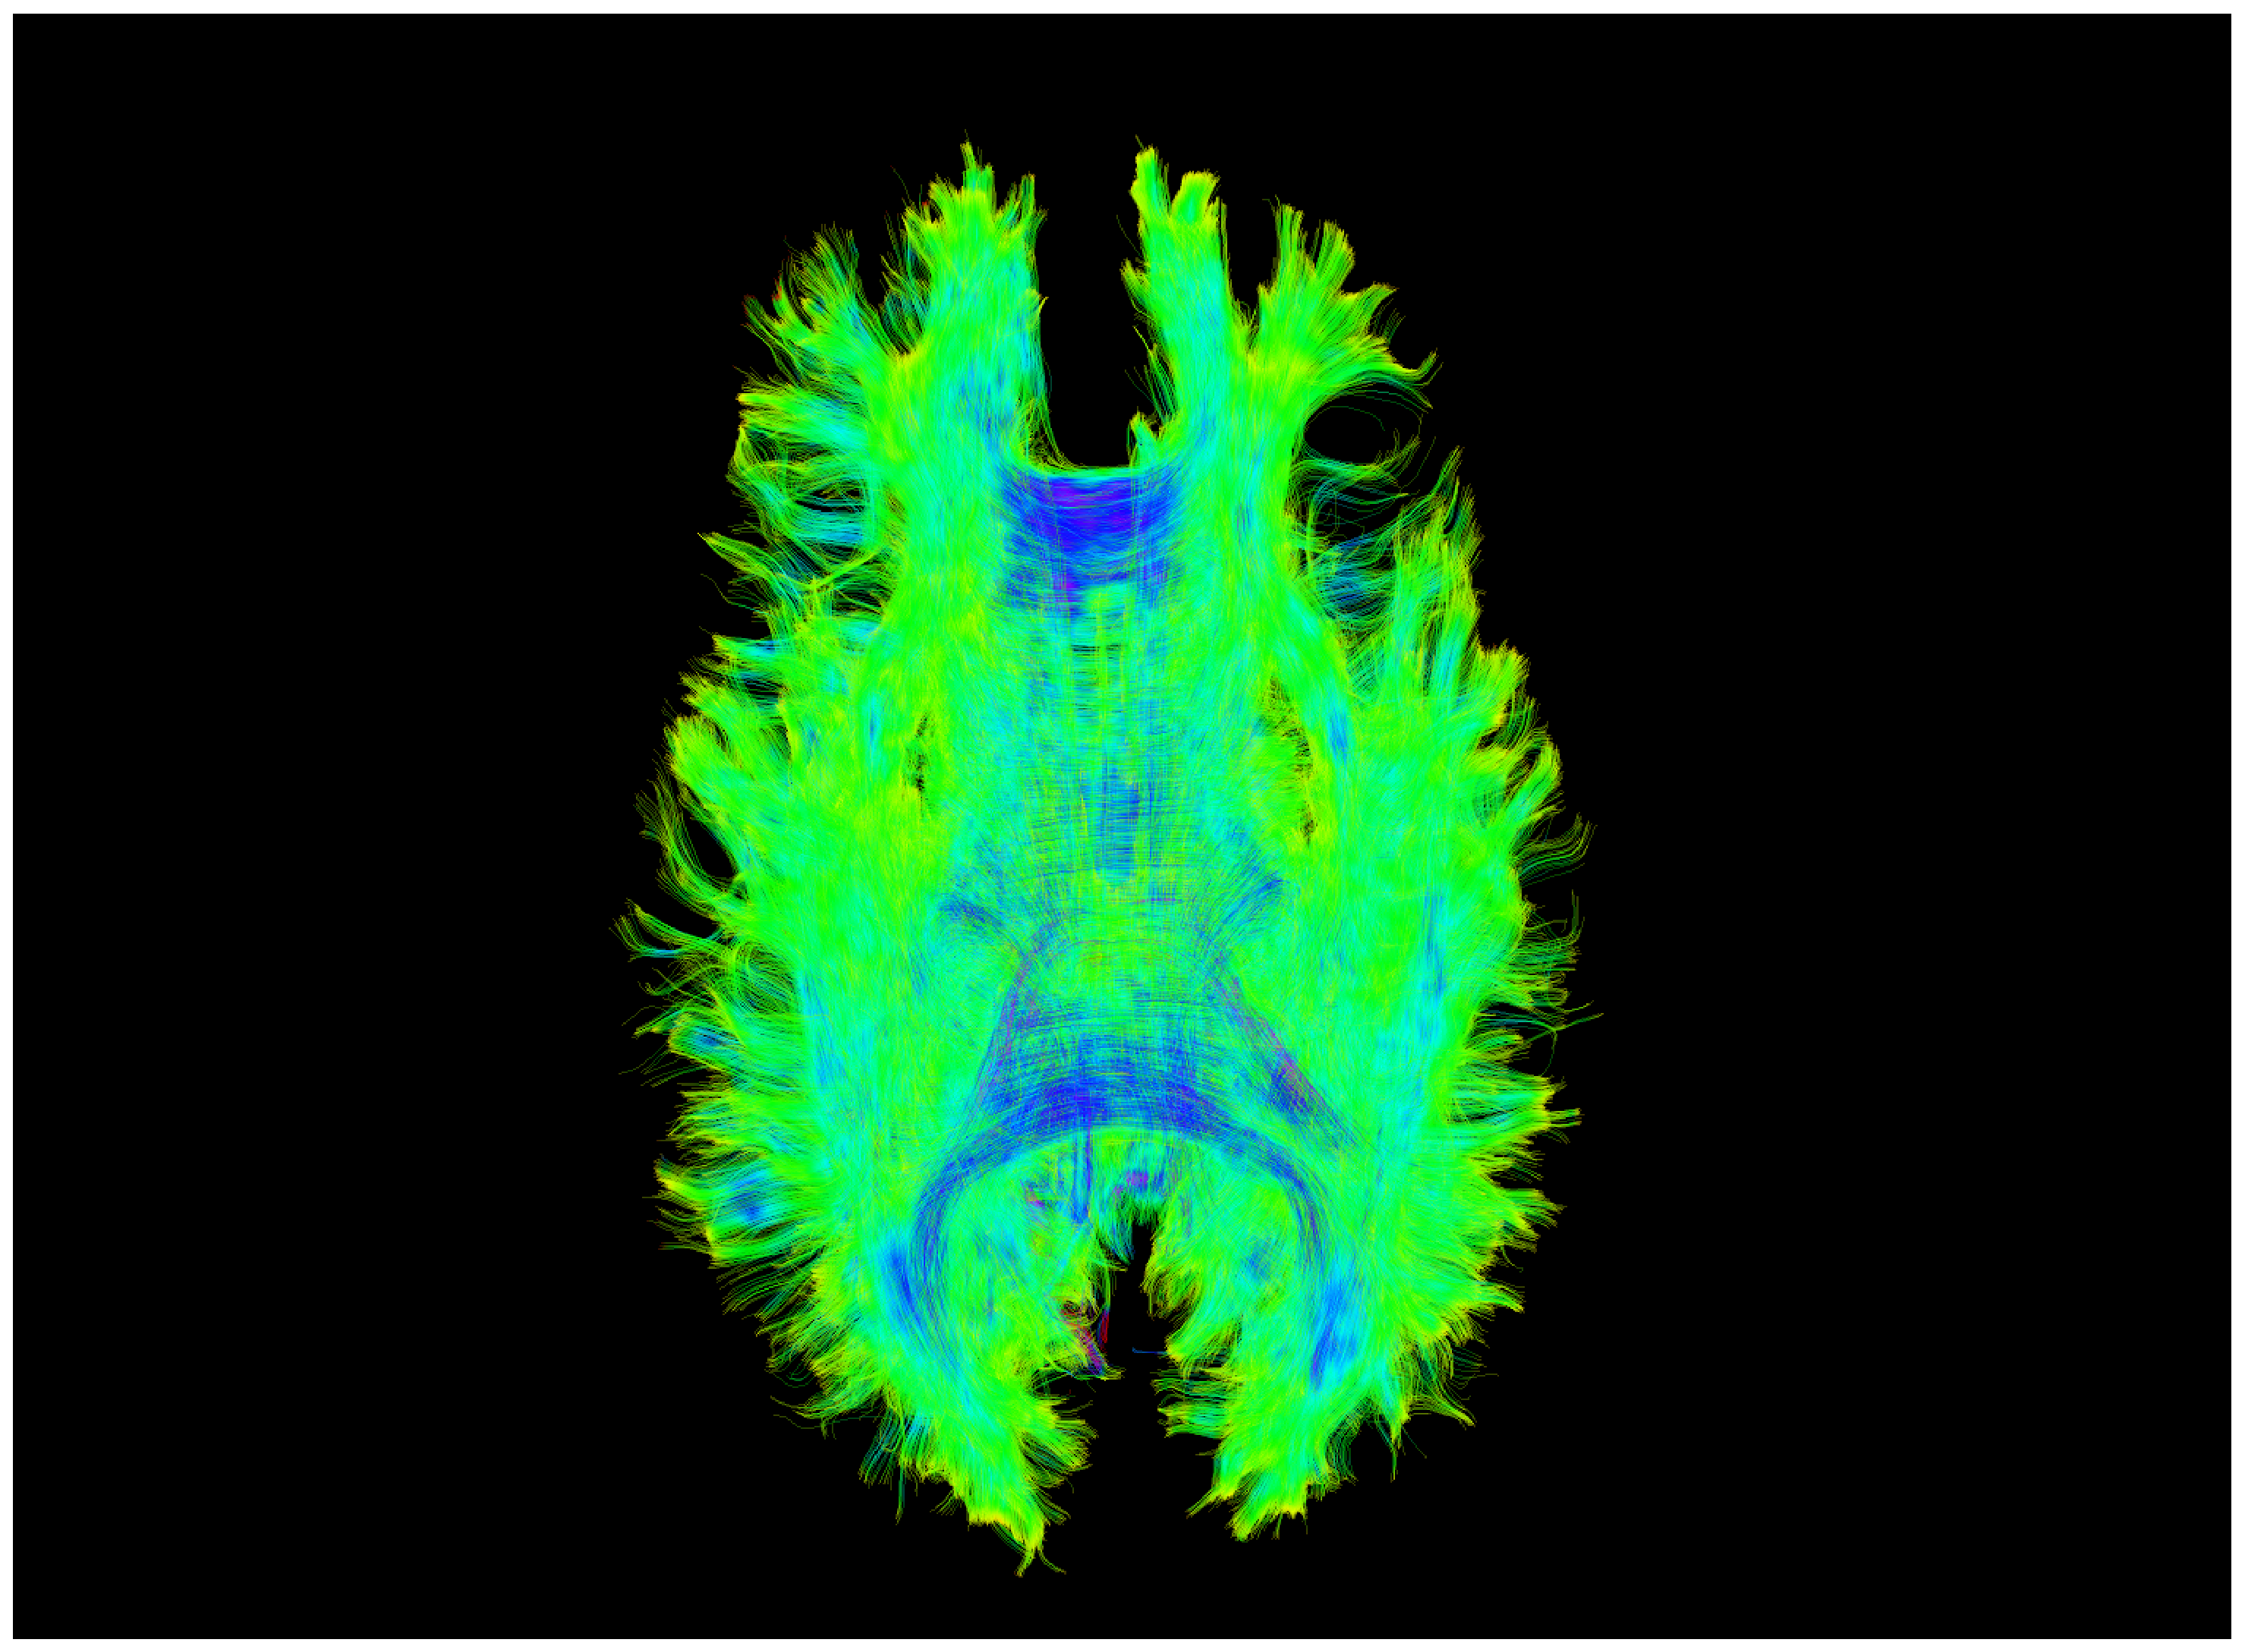
\includegraphics[width=4cm]{Tarctography1-Interior-View}

        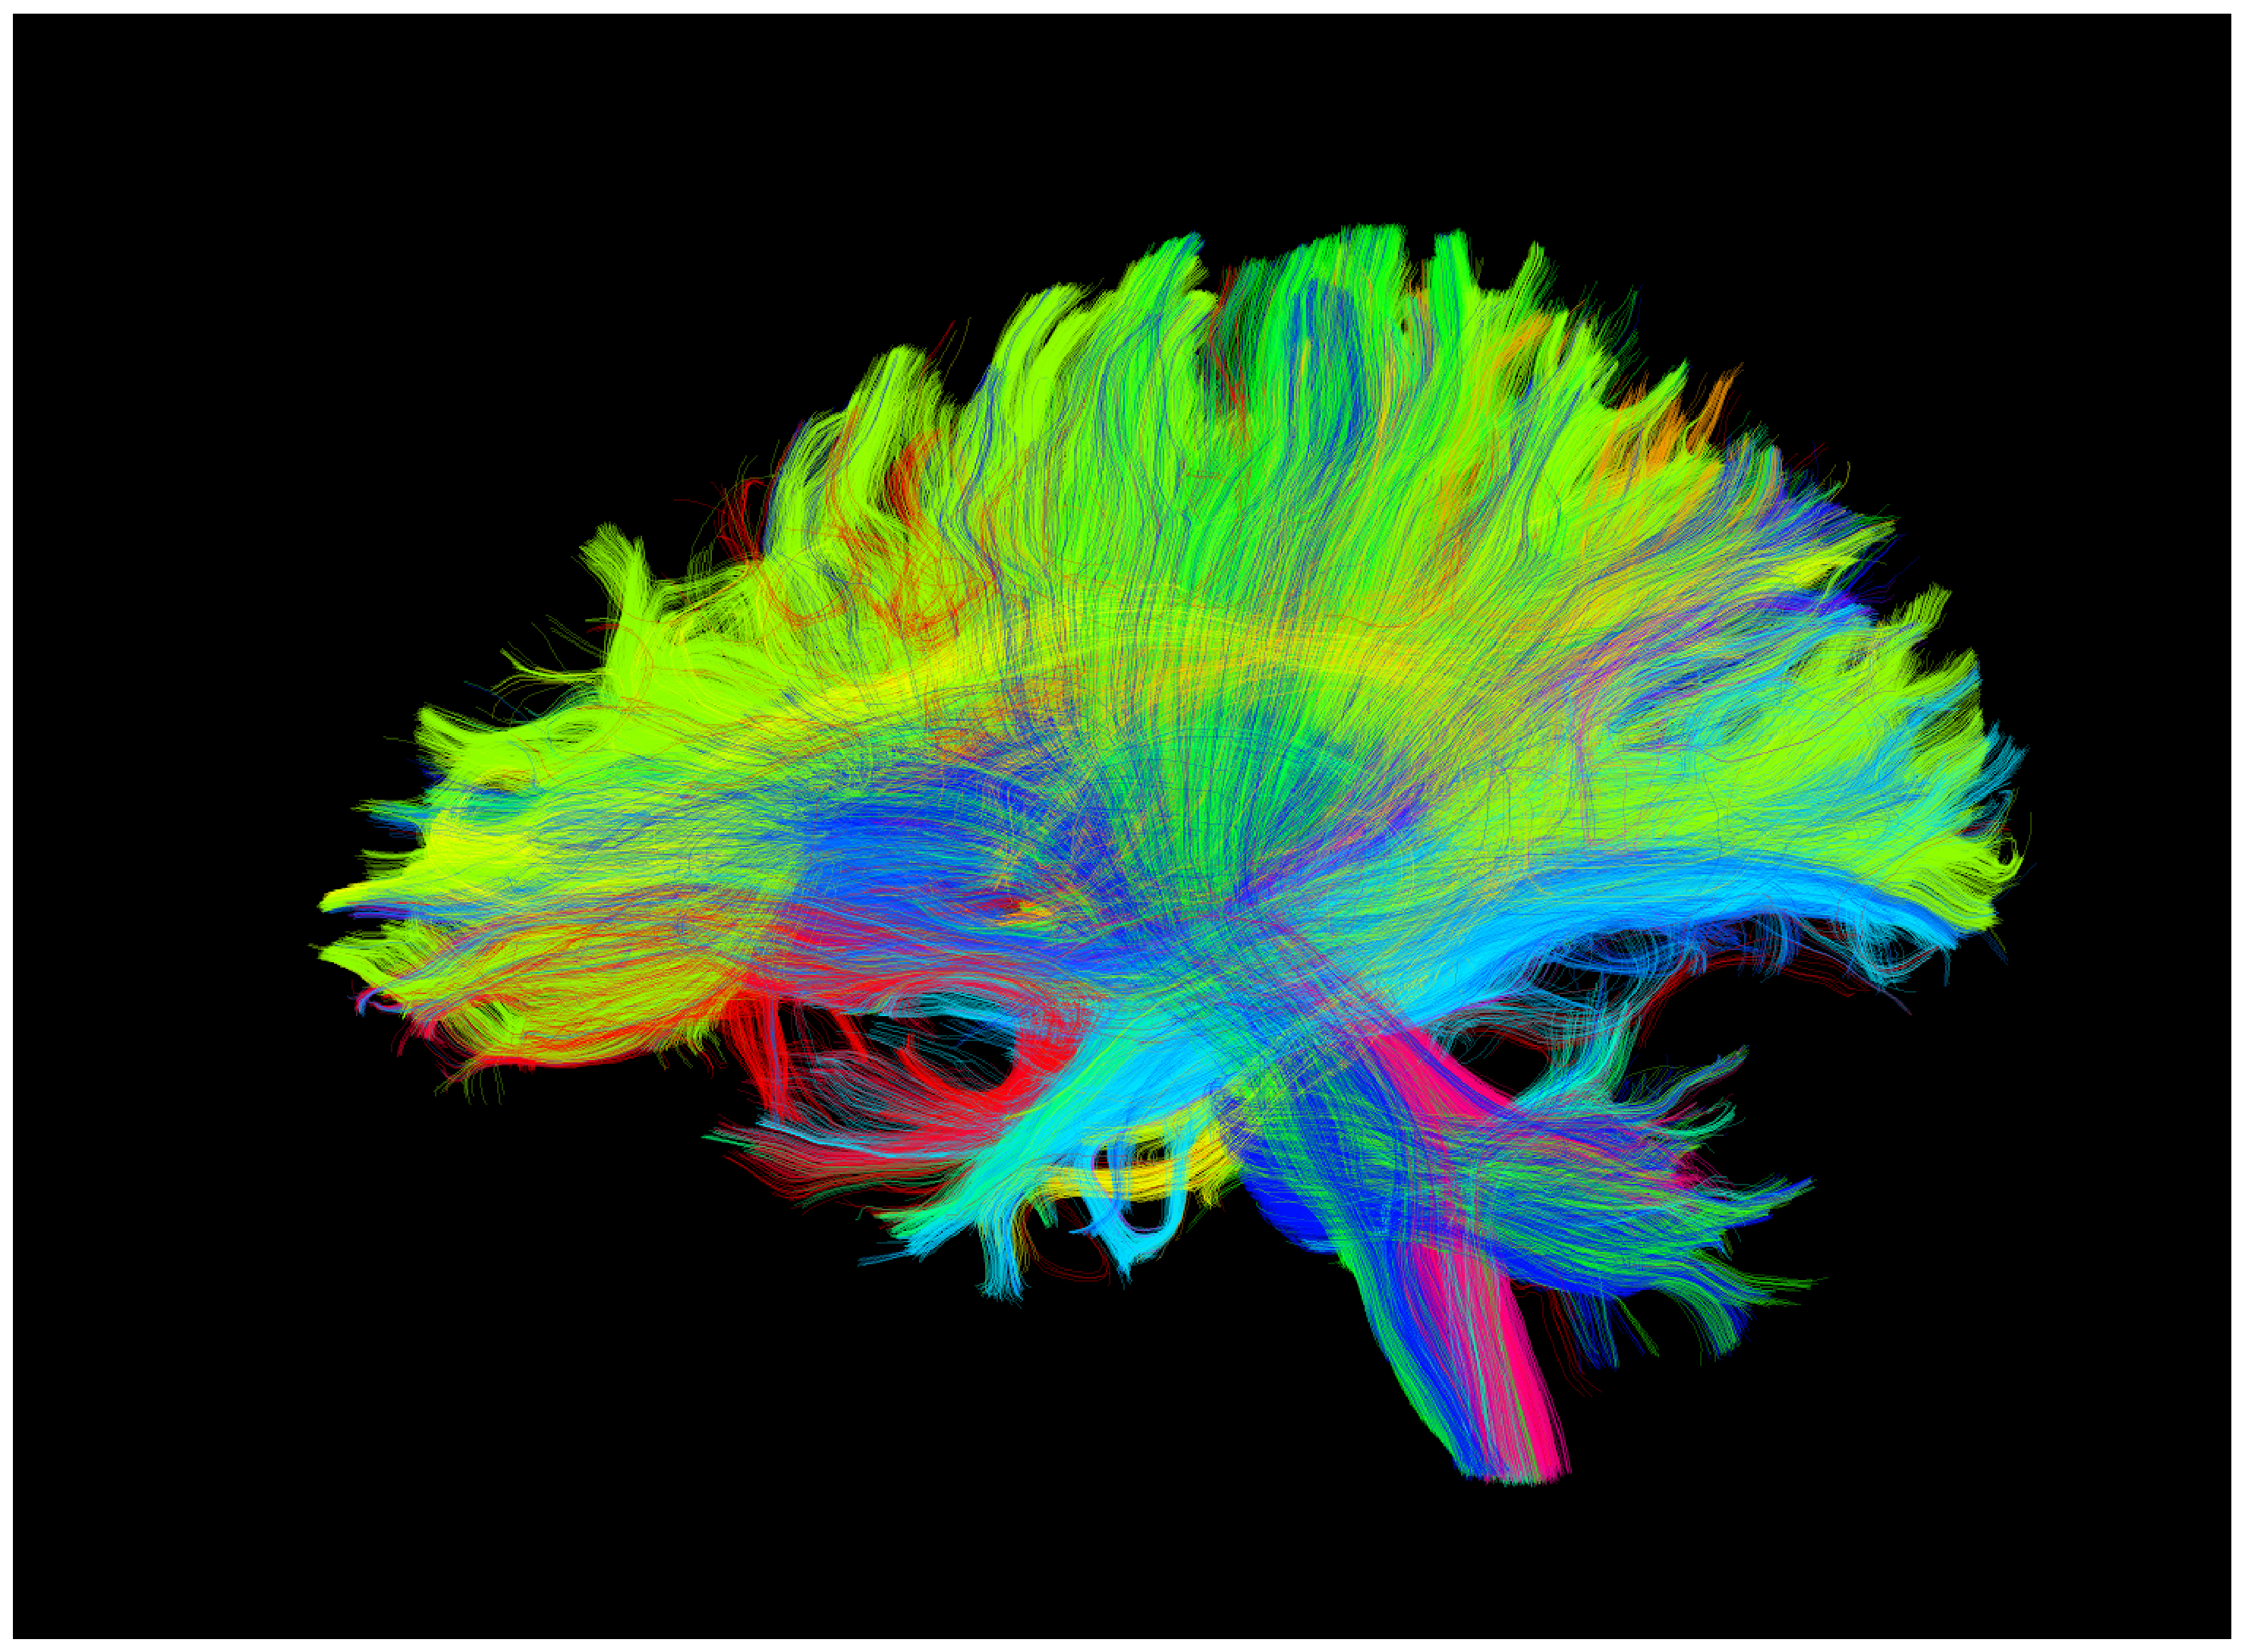
\includegraphics[width=4cm]{Clustering1-Left-View}
        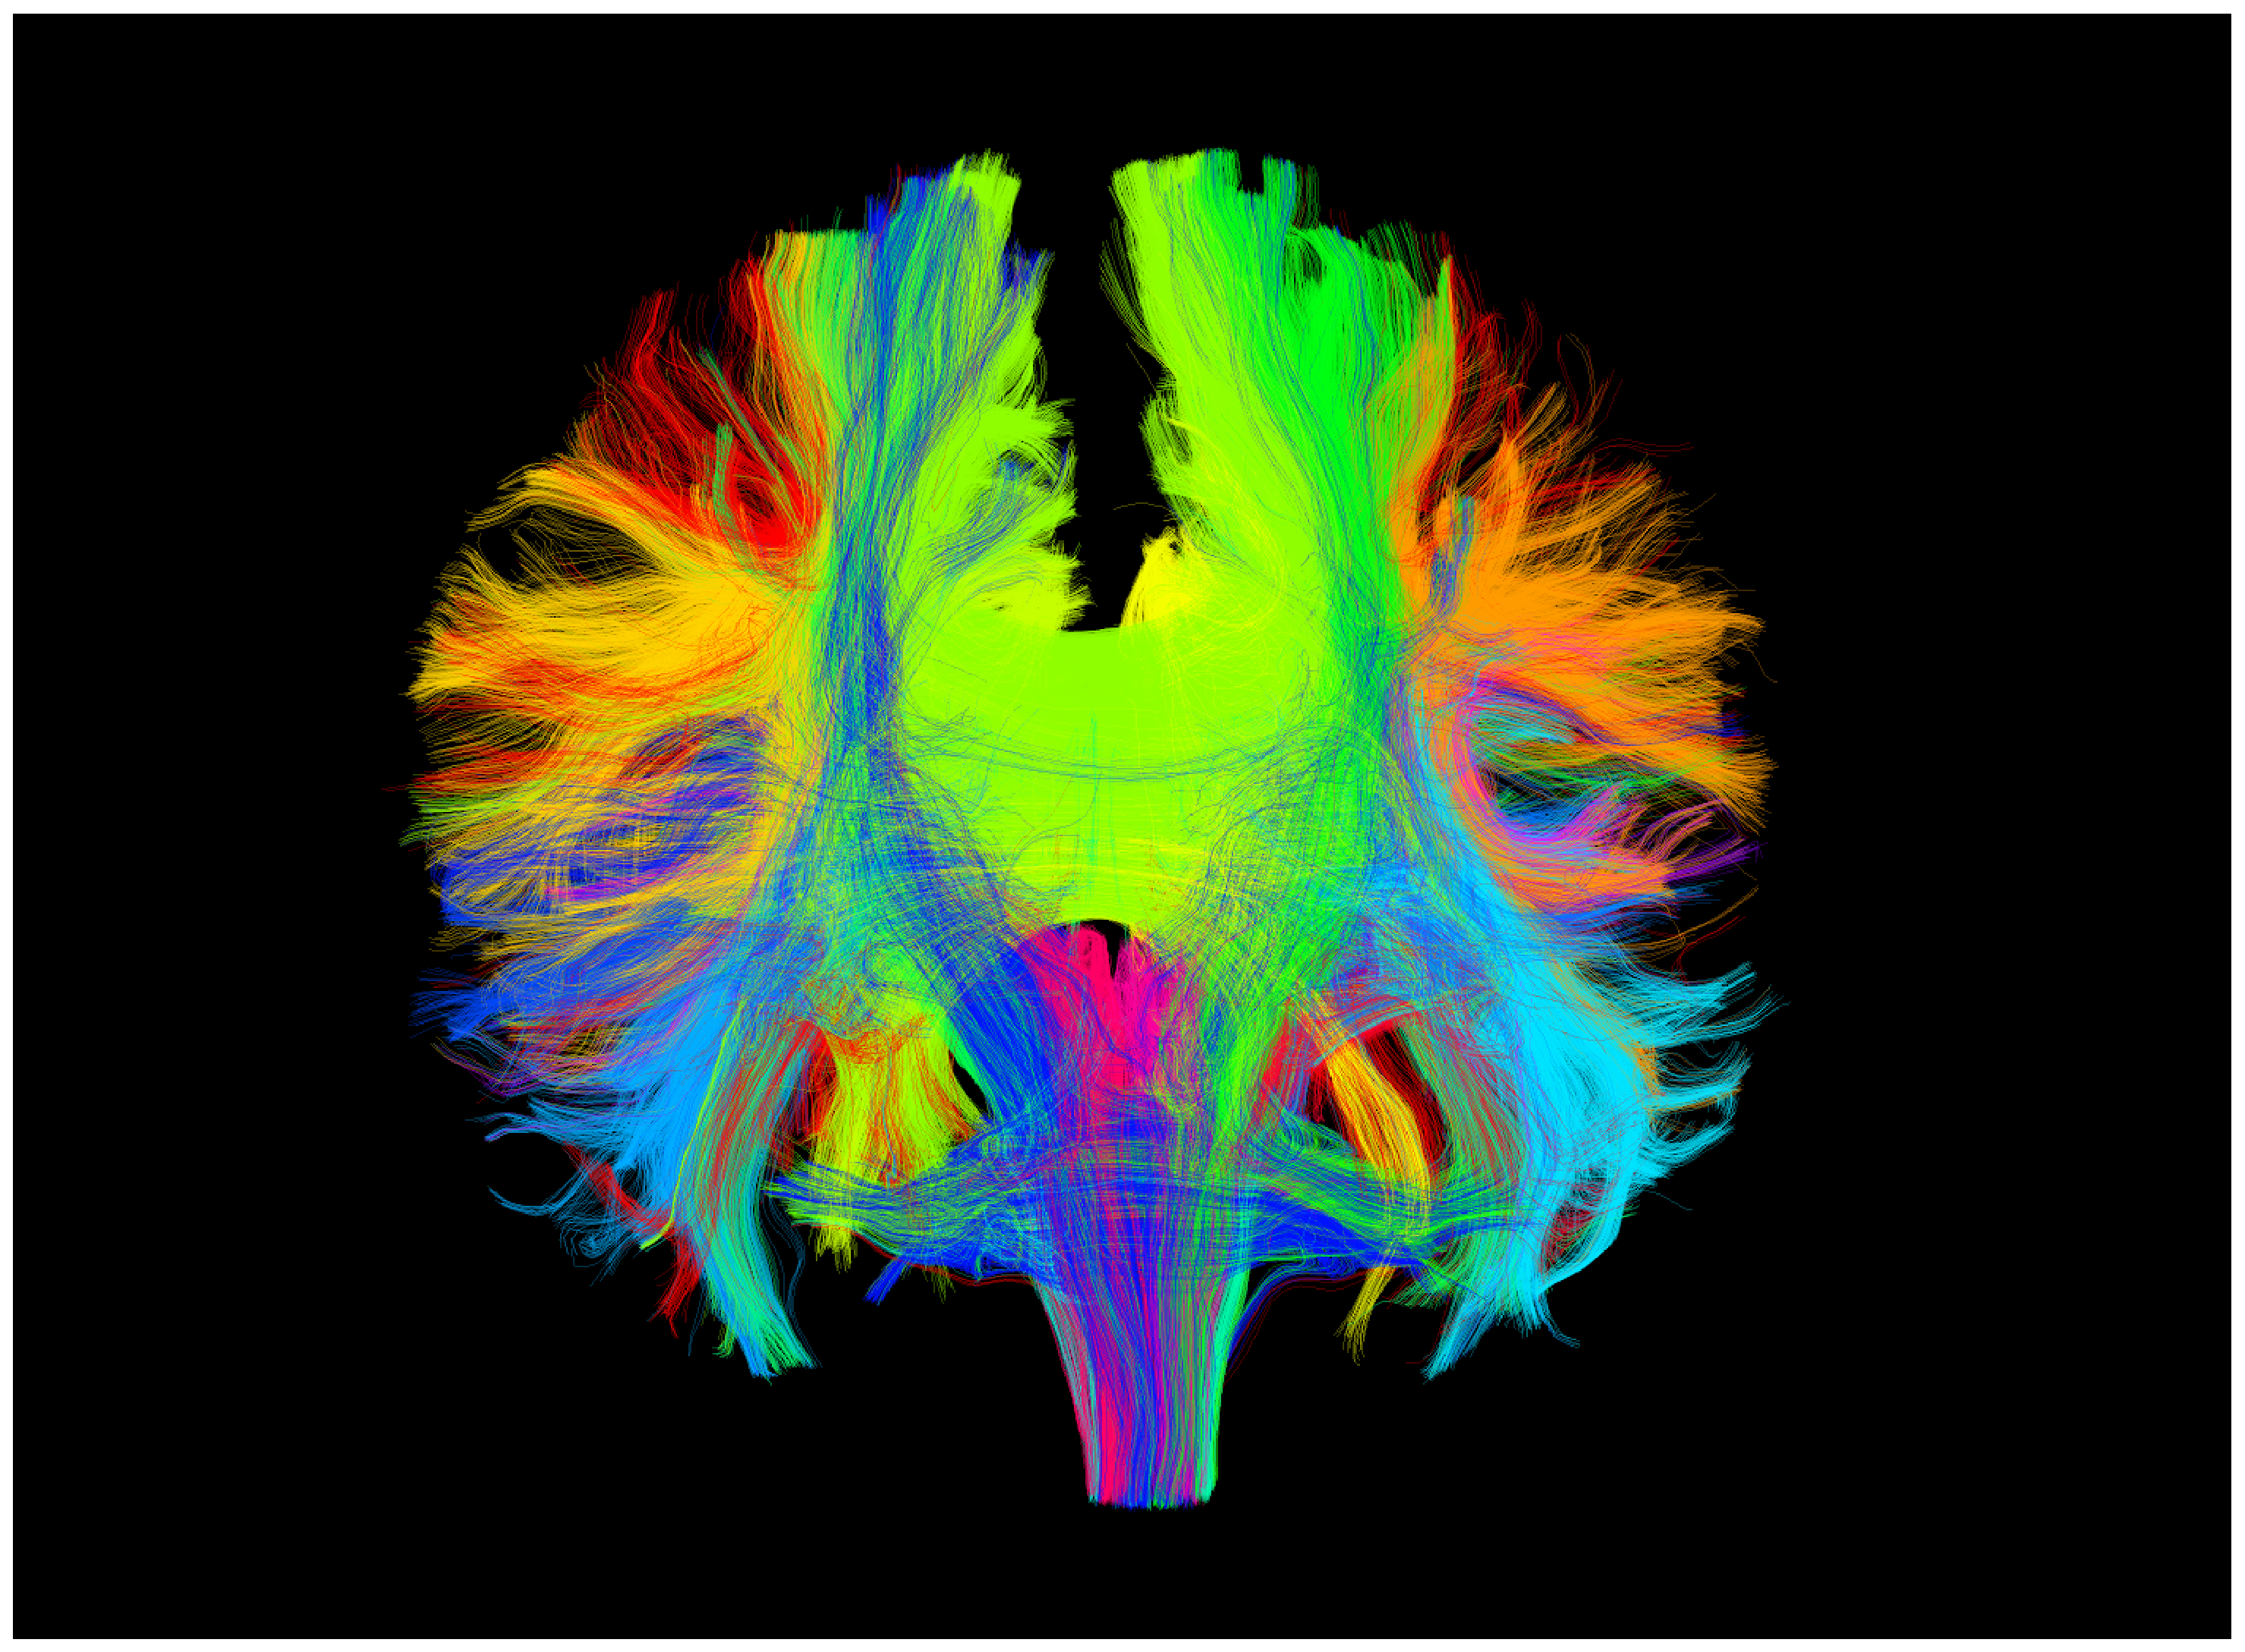
\includegraphics[width=4cm]{Clustering1-Anterior-View}
        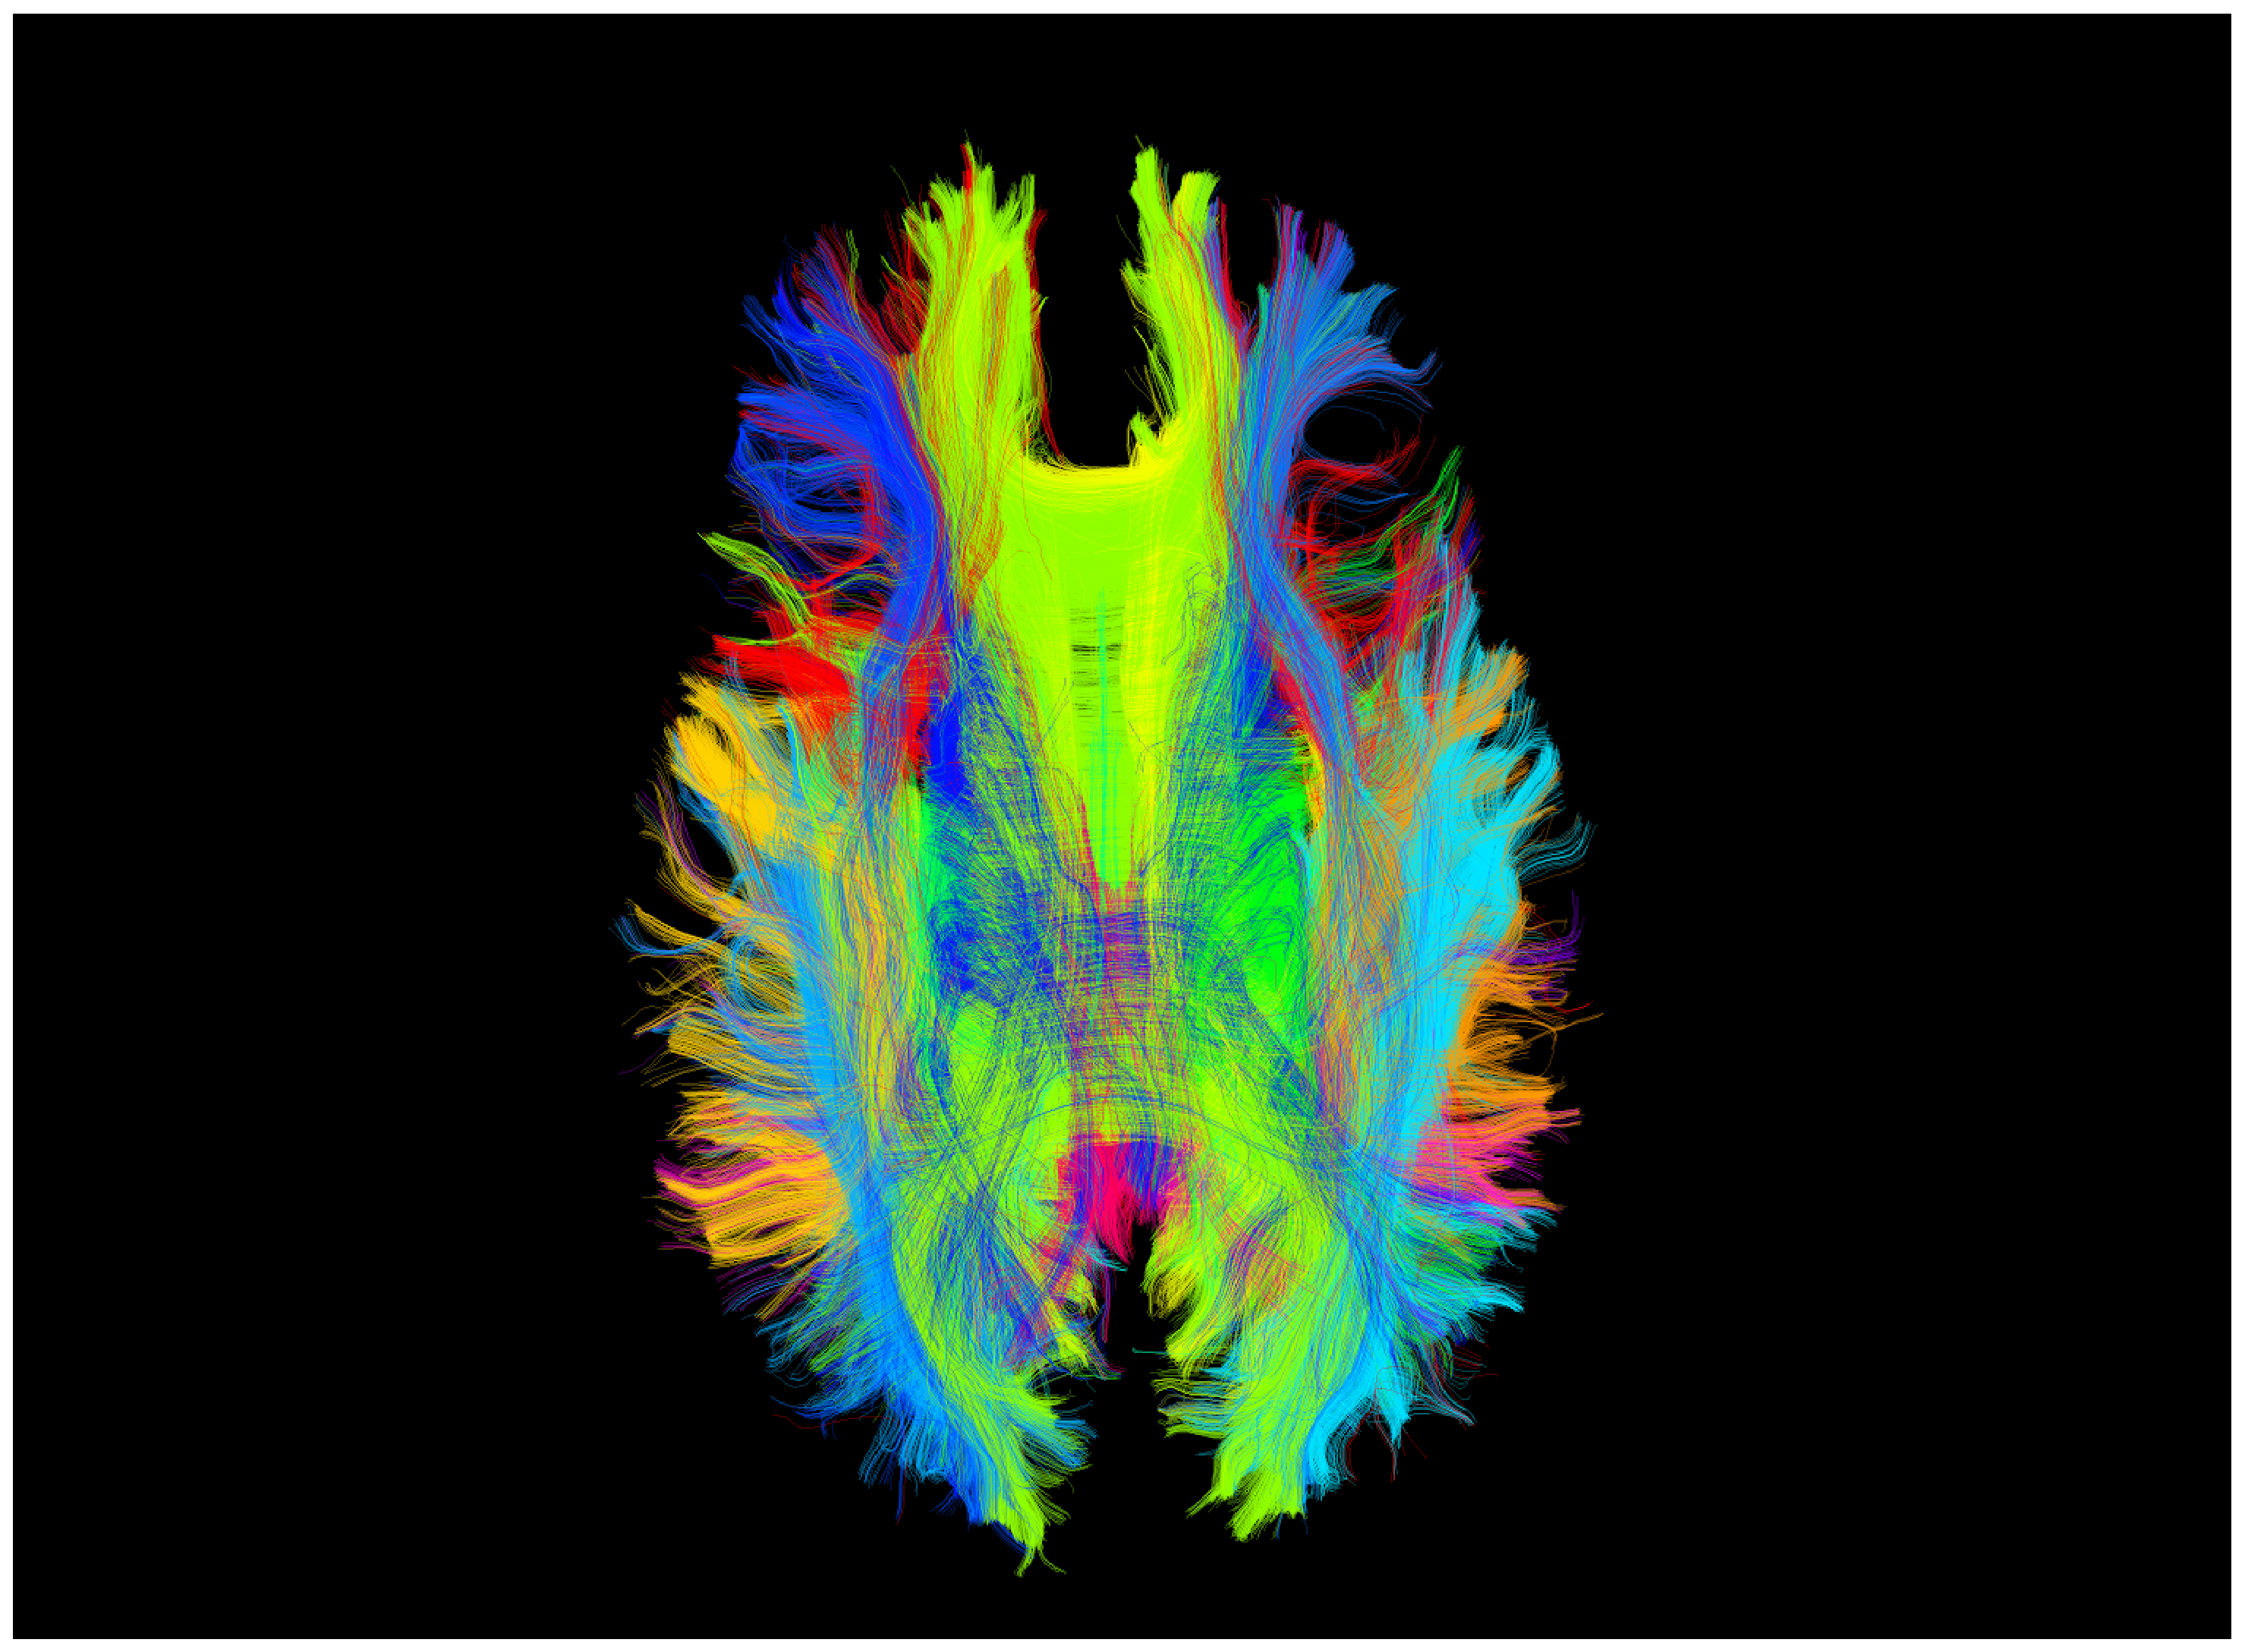
\includegraphics[width=4cm]{Clustering1-Interior-View}

        \caption{An example of fiber tracts clustering in the whole brain using \texttt{btkProbabilisticSegmentationMapBasedClustering} method.
        {\em The fibers from the tractography process and final clustering fiber bundles are shown in the first and second row, respectively. Three viewing angles of 3D depictions of fibers are shown (from left to right): left lateral view, anferior view and interior view. }}
        \label{clustering1-fig}
        \end{figure}

	\item[btkDistanceFibersKMeansApproximationClustering] As unsupervised method, this program makes it possible to cluster the fibers according to their anatomical regions using a distance metric based on the similarity between fibers.\\

	Usage: \texttt{btkDistanceFibersKMeansApproximationClustering -b fiber\_tractography.vtk -d distance\_measure -c number\_of\_clusters -o fiber\_clustering.vtk} \\

	The full list of optional parameters of this method can be obtained by:\\ 
        \texttt{btkDistanceFibersKMeansApproximationClustering --help}

	Fig.\ref{clustering2-fig} shows an example of clustering results in the corpus callosum region obtained using the method above with the following input parameters: \texttt{-d 10 -c 7}.

	\begin{figure}[h]
	\centering
        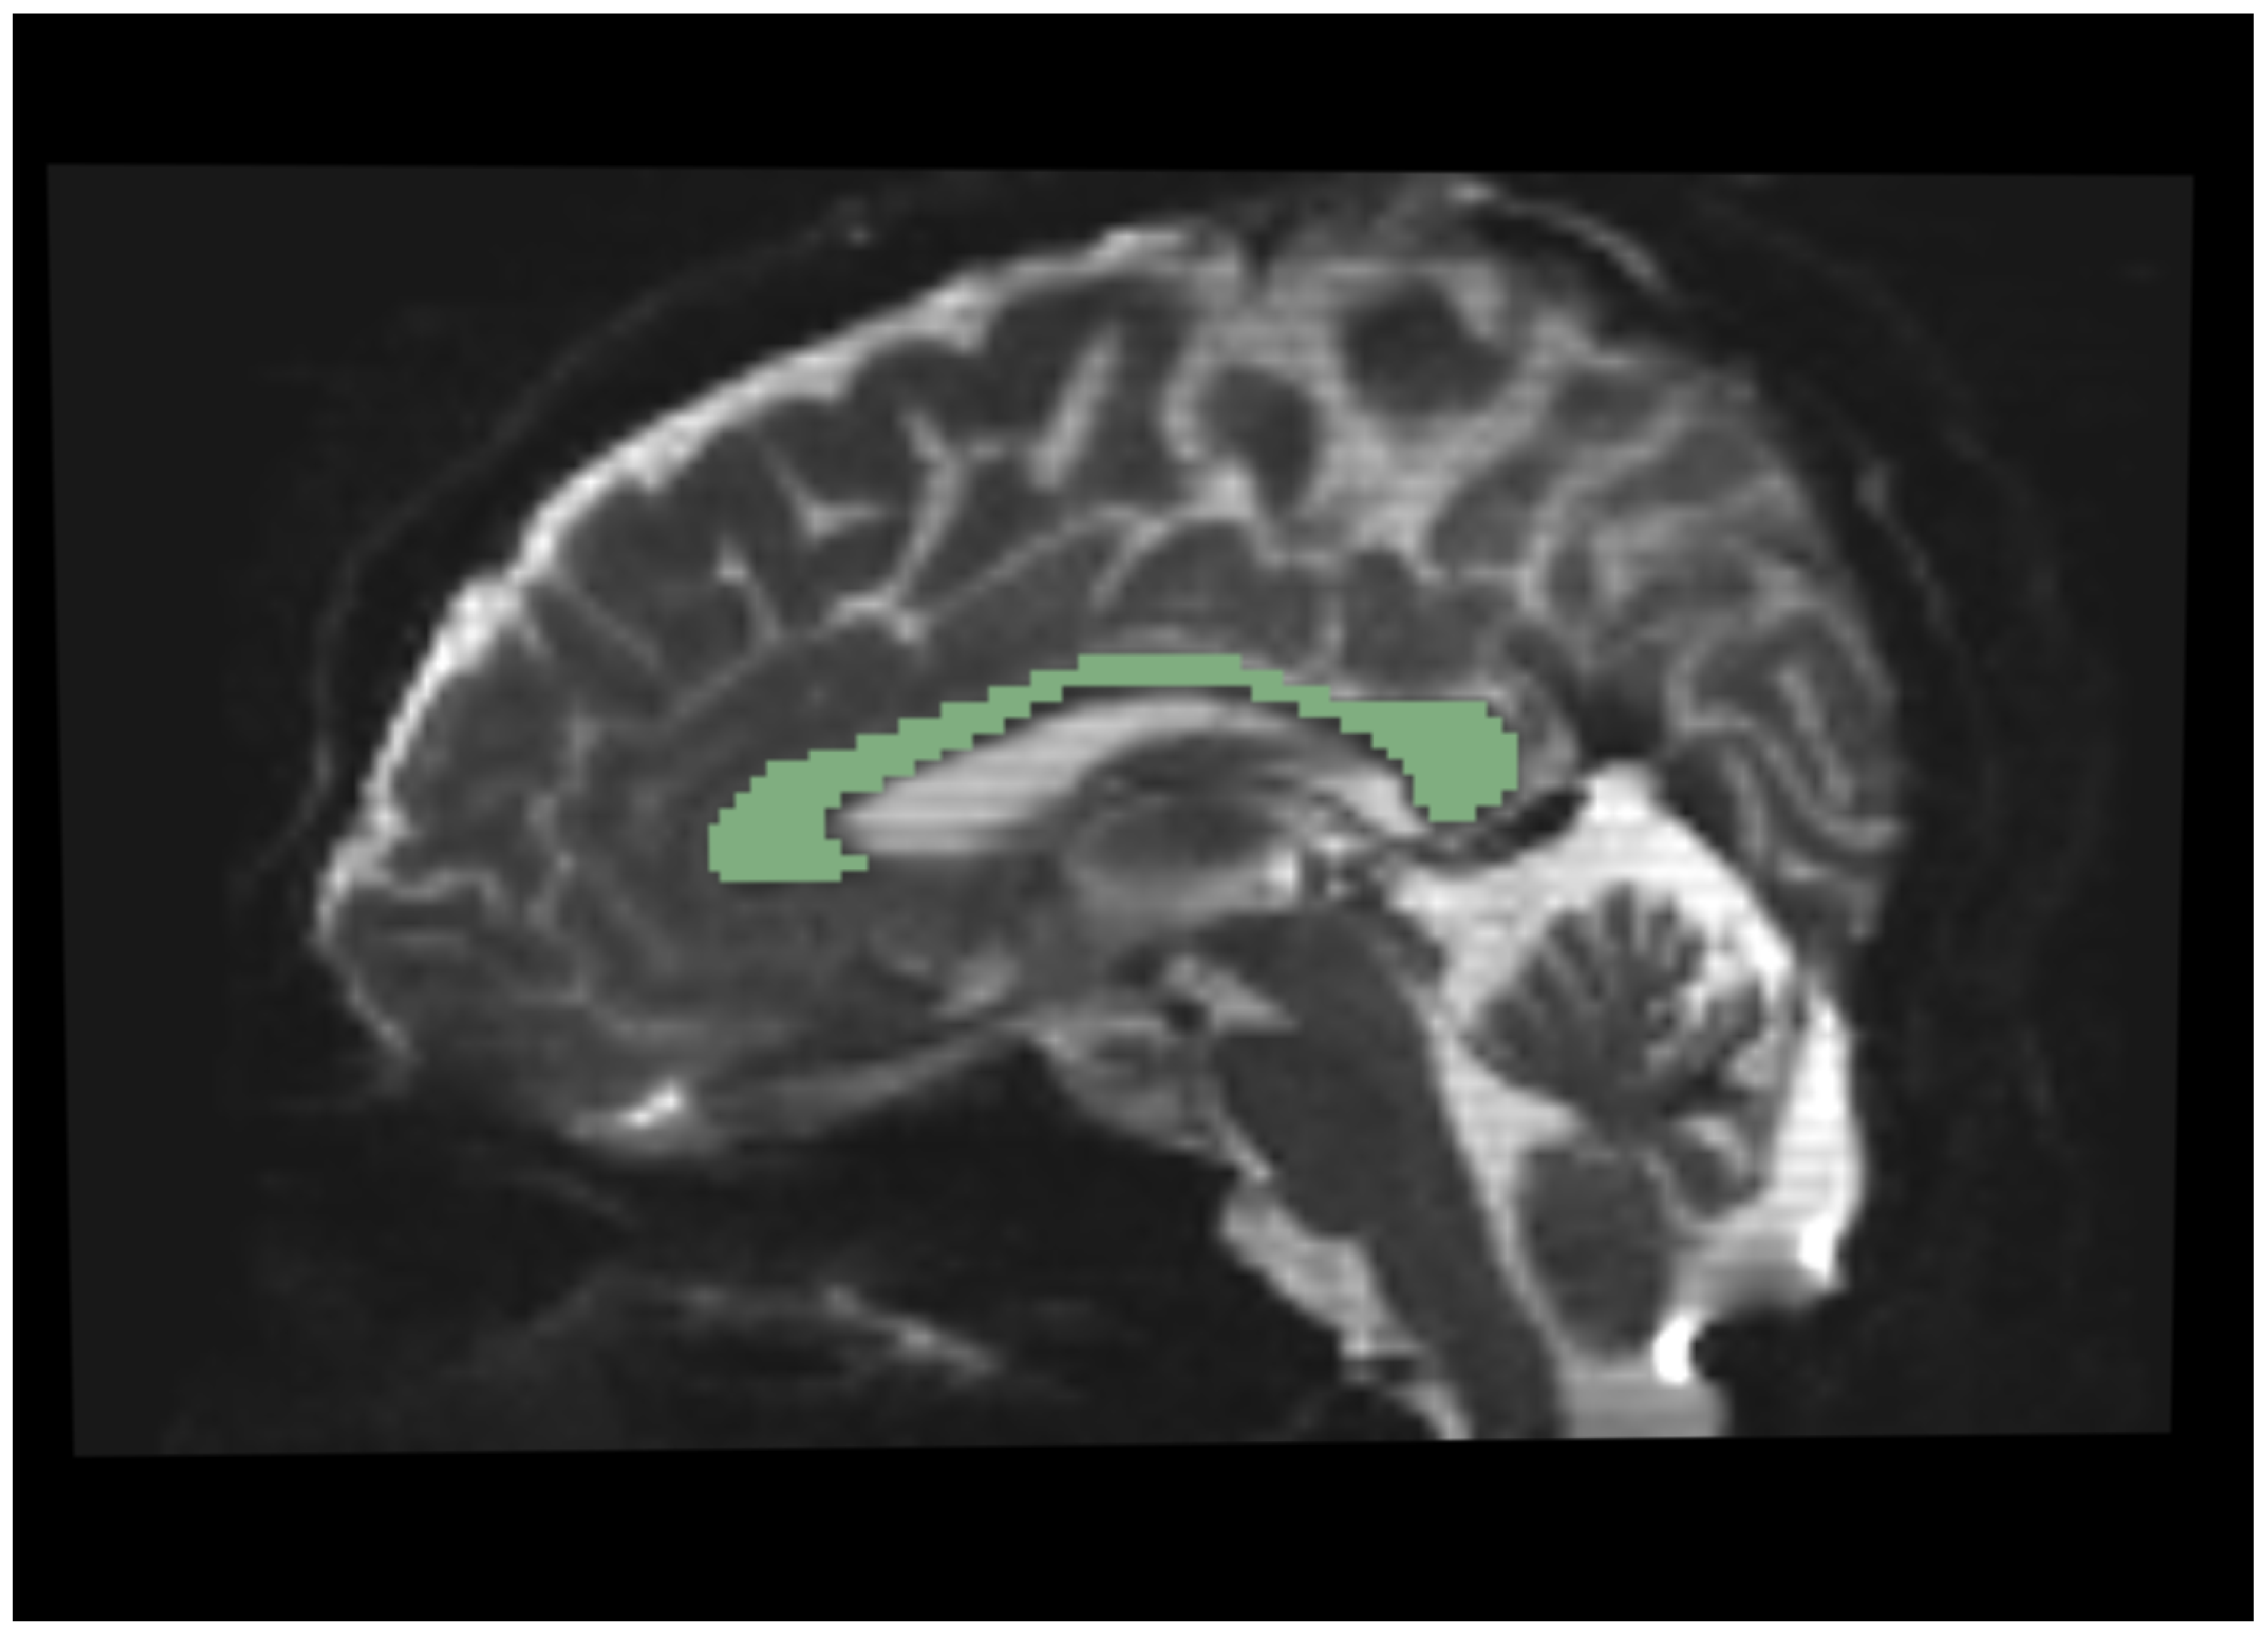
\includegraphics[width=4cm]{Corpus_Callosum-view2}
        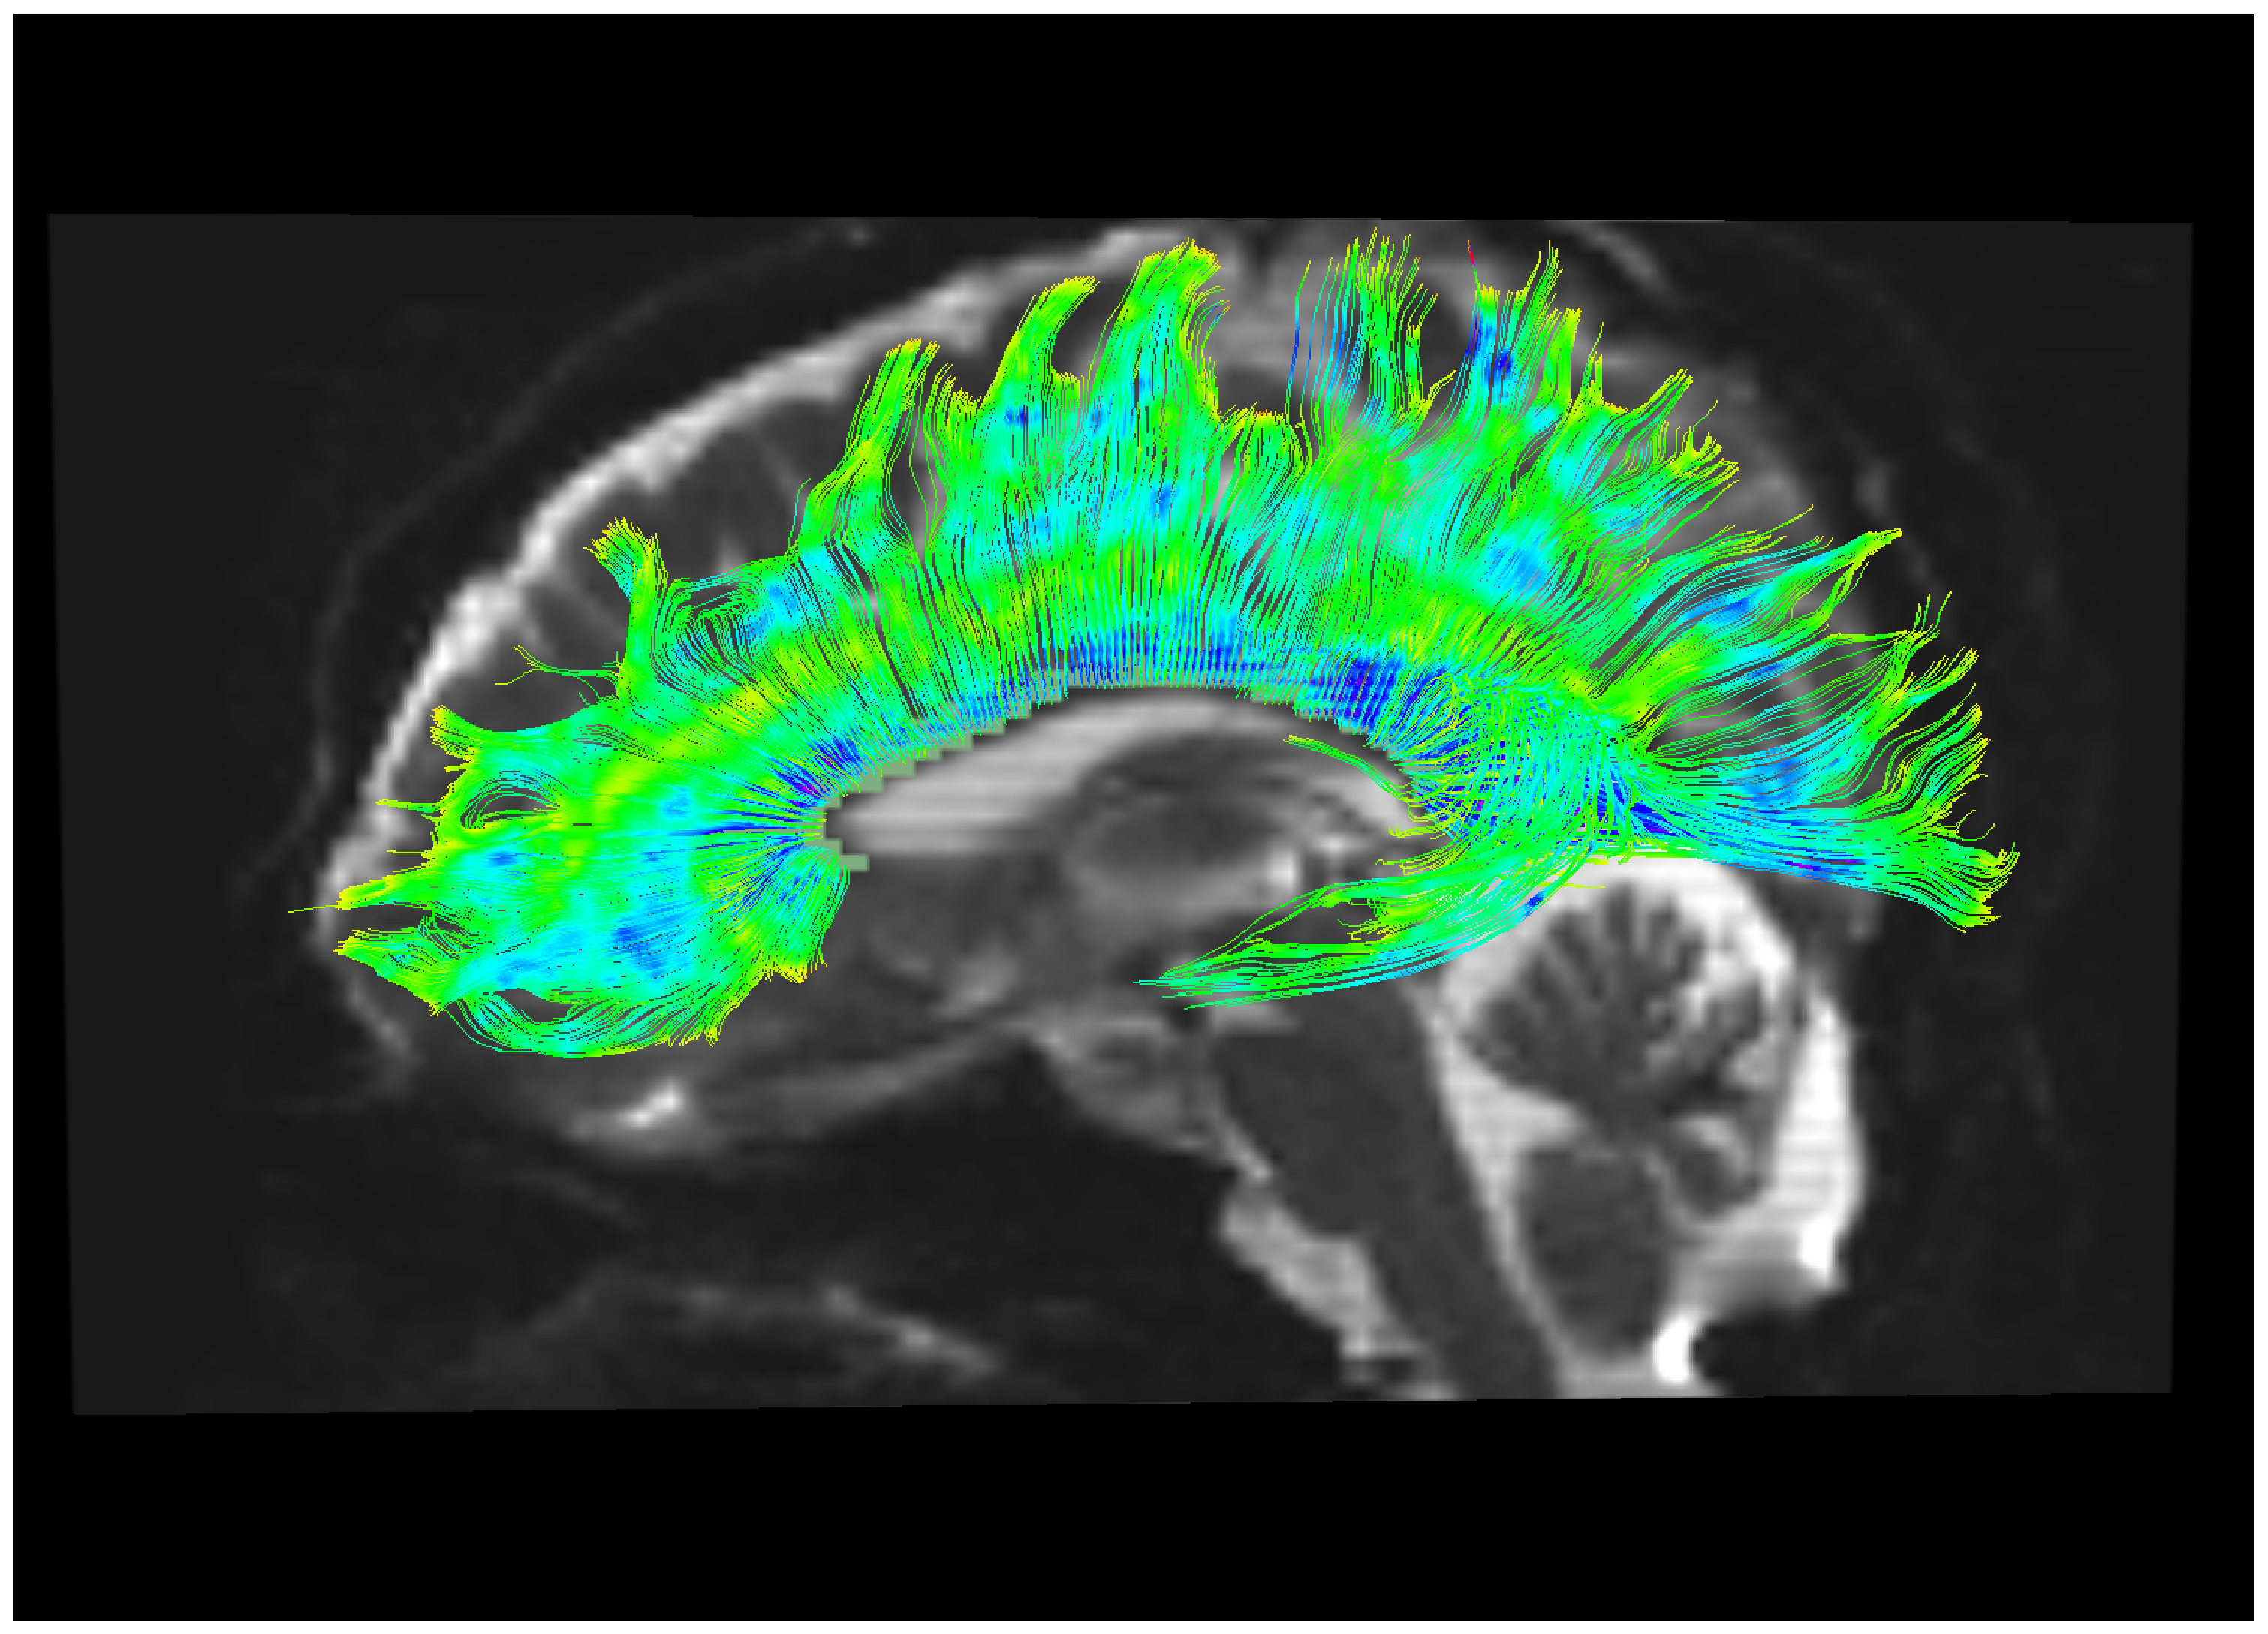
\includegraphics[width=4cm]{Tractography-CC-view2}
        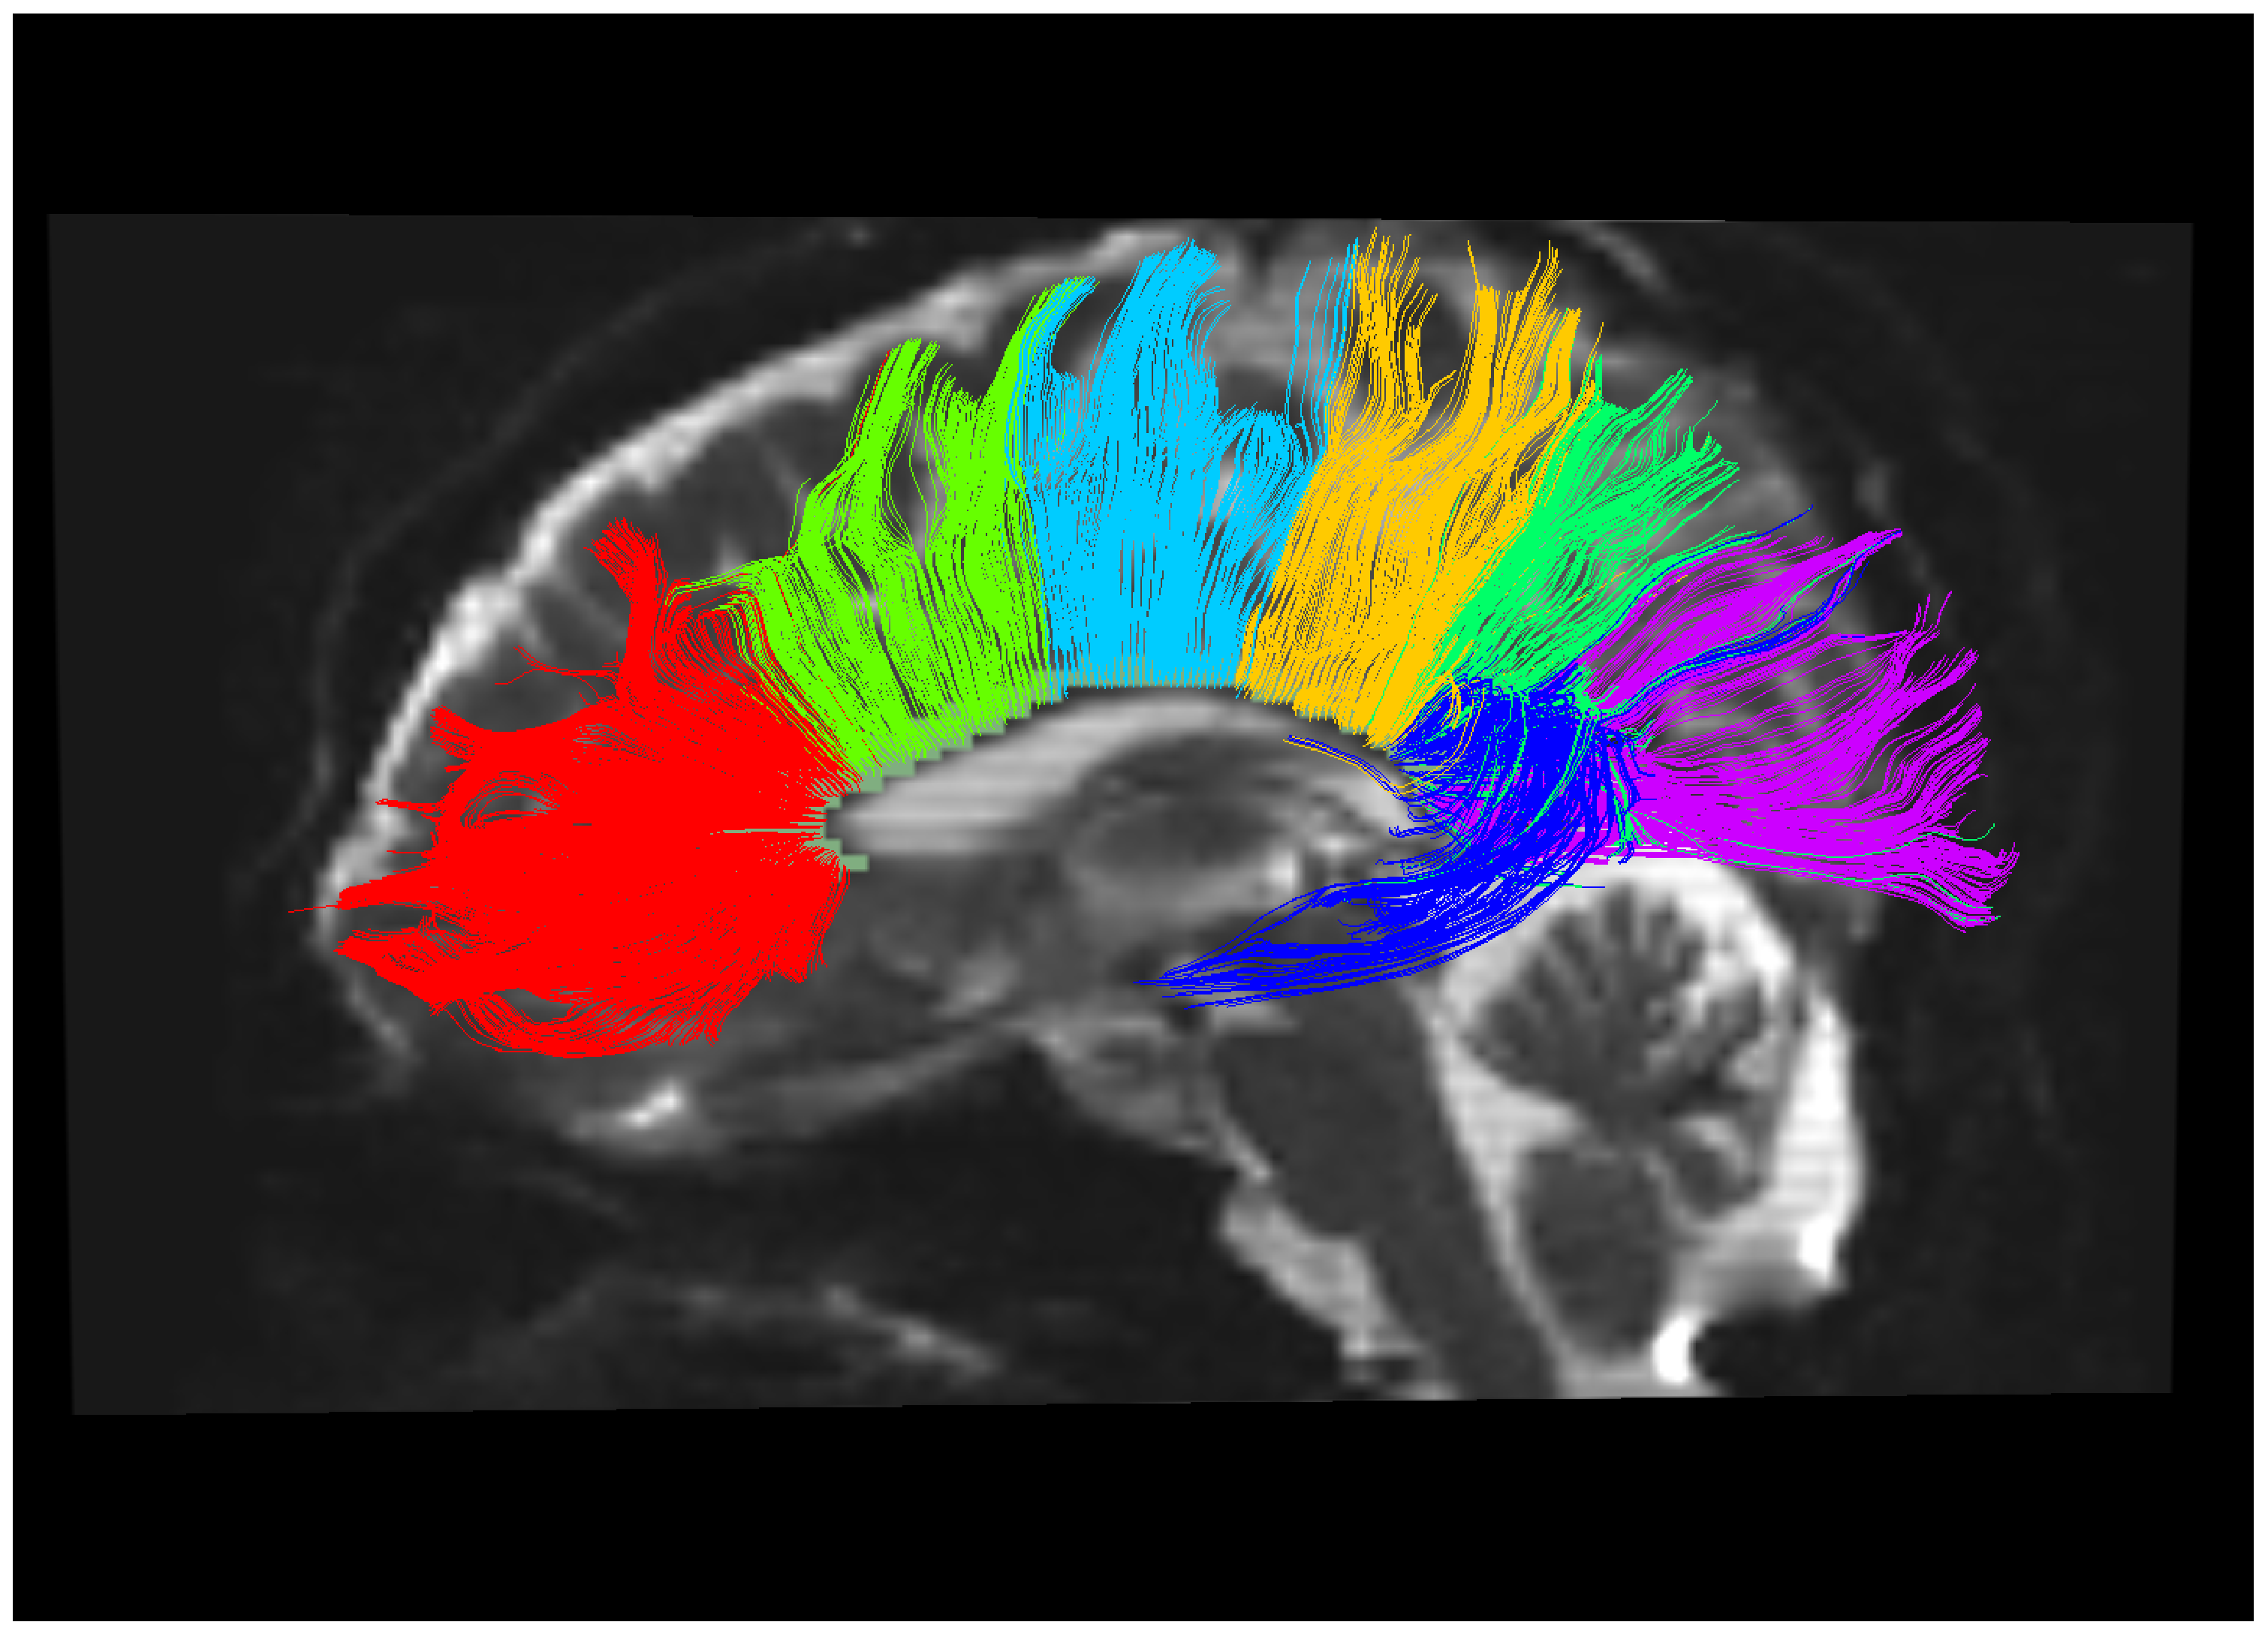
\includegraphics[width=4cm]{Clustering2-CC-view2}
        \caption{An example of fiber tracts clustering in the corpus callosum using \texttt{btkProbabilisticSegmentationMapBasedClustering} method.
        {\em The region of interest on the corpus callosum, fibers from the tractography process and final clustering fiber bundles are shown from left to right, respectively. The fibers are clustered according to anatomical regions as proposed by \href{brain.oxfordjournals.org/content/112/3/799}{Witelson}.}}
        \label{clustering2-fig}
        \end{figure}

\end{description}
